%
%  Thesis template for Heilbronn University of Applied Sciences
%
%  Created by Prof. Dr. Detlef Stern on 2010-08-14.
%  Updated by Valentin Weber on 2020-10-05.
%  Copyright (c) 2020 . All rights reserved.
%
\documentclass[12pt,toc=bib,toc=listof]{scrreprt}
\usepackage[english]{babel} 
\usepackage{mathptmx,amsmath,mathtools}

% Declare acronyms
\usepackage{acro}

\DeclareAcronym{VR}{
  short = VR,
  long  = Virtual Reality
}
\DeclareAcronym{TAM}{
  short = TAM,
  long  = Technology Acceptance Model
}
\DeclareAcronym{HP}{
  short = HP,
  long  = Head Pointing
}
\DeclareAcronym{GPU}{
  short = GPU,
  long  = Graphics processing unit
}
\DeclareAcronym{FH}{
  short = FH,
  long  = Free Hand
}
\DeclareAcronym{CP}{
  short = CP,
  long  = Control Pointing
}
\DeclareAcronym{DC}{
  short = DC,
  long  = Discrete Cursor
}
\DeclareAcronym{CC}{
  short = CC,
  long  = Continuous Cursor
}
\DeclareAcronym{WPM}{
  short = WPM,
  long  = Words Per Minute
}
\DeclareAcronym{ER}{
  short = ER,
  long  = Error Rate
}
\DeclareAcronym{HCI}{
  short = HCI,
  long  = Human-Computer Interaction
}
\DeclareAcronym{AI}{
  short = AI,
  long  = Artificial Intelligence
}
\DeclareAcronym{ML}{
  short = ML,
  long  = Machine Learning
}
\DeclareAcronym{AHAP}{
  short = AHAP,
  long  = Apple Haptic Programming
}



\DeclareAcronym{HMD}{
  short = HMD,
  long  = Head-Mounted Display
}
\DeclareAcronym{DoF}{
  short = DoF,
  long  = Degrees of Freedom
}
\DeclareAcronym{LCD}{
  short = LCD,
  long  = Liquid Crystal Display
}
\DeclareAcronym{OLED}{
  short = OLED,
  long  = Organic Light Emitting Diode
}
\DeclareAcronym{AMOLED}{
  short = AMOLED,
  long  = Active Matrix Organic Light Emitting Diode
}

\DeclareAcronym{SDK}{
  short = SDK,
  long  = Software Development Kit
}

\DeclareAcronym{UI}{
  short = UI,
  long  = User Interface
}
\DeclareAcronym{XR}{
  short = XR,
  long  = Extended Reality
}
\DeclareAcronym{FFB}{
  short = FFB,
  long  = Force Feedback
}
\usepackage[utf8]{inputenc}
\usepackage[T1]{fontenc}
\usepackage{lmodern}
\usepackage{setspace}
\usepackage{geometry}
\usepackage{lettrine}
\usepackage{subcaption}

\usepackage{hyperref}
\hypersetup{
  ,colorlinks=true
  ,linkcolor=blue
  ,citecolor=blue
  ,filecolor=blue
  ,urlcolor=blue
  }
\usepackage{caption}

% Subject related values (need updating)
\newcommand{\hhnsubject}{SUBJECT}
\newcommand{\hhnsubjectnum}{SPO NUMBER}
\newcommand{\hhnlecturer}{LECTURER}

% Student related values (need to be updated)
\newcommand{\reprttopic}{ \centering Enhancing User Experience and Productivity in \ac{VR} Programming Environments}
\newcommand{\reprtstudentname}{KHEIREDDINE AZZEZ}
\newcommand{\reprtstudentid}{215021}
\urldef{\reprtstudentmail}\url{kazzez@stud.hs-heilbronn.de}

\usepackage{ifpdf}
\ifpdf
\usepackage[pdftex]{graphicx}
\else
\usepackage{graphicx}
\fi

\usepackage[headsepline]{scrlayer-scrpage}
\usepackage{pdfpages} % Add this package
\usepackage{lscape} 

\pagestyle{scrheadings}
\clearscrheadfoot
\ihead{\hhnsubject: \reprttopic}
\ohead{ \\ \pagemark}
\renewcommand*{\chapterpagestyle}{scrheadings}
\renewcommand*{\chapterheadstartvskip}{}

% title page definition (begin)
\titlehead{\flushright
\includegraphics{graphics/hhn_en.png}}
\subject{{\hhnsubject{} (\hhnsubjectnum{})}}
\title{\reprttopic}
\author{\reprtstudentname\footnote{\reprtstudentid, \reprtstudentmail}}
%% Never set date to a specific value
\publishers{Submitted to \hhnlecturer}
% title page definition (end)
\begin{document}
\pagenumbering{Roman} 
\selectlanguage{english}
\maketitle
\newgeometry{left=30mm, top=25mm, right=15mm, bottom=25mm}

\tableofcontents
\chapter*{List of Abbreviations}
\addcontentsline{toc}{chapter}{List of Abbreviations}
\printacronyms[heading=none, display=all]

\label{sec:listofabbrv}
% chapter listofabbrv (end)

\listoffigures
\listoftables

\onehalfspacing

\addchap{Management Summary} % (fold)
\label{cha:management_summary}

This thesis investigates the enhancement of user experience and productivity within \ac{VR} programming environments, focusing particularly on the integration of advanced \ac{FFB} and optimized virtual keyboard design. As \ac{VR} technologies evolve, there is a growing need to create more intuitive and immersive interaction systems that mimic the real-world experience as closely as possible.\\ \\
The study explores various methodologies for improving \ac{VR} interfaces, particularly through the implementation of dynamic and adaptive \ac{FFB} systems that provide users with realistic tactile responses. This approach aims to increase the naturalness of interactions in \ac{VR}, making them feel more intuitive and less fatiguing, which is critical for productivity in programming and other detailed-oriented tasks.\\ \\
A significant portion of the research is dedicated to the development of a virtual keyboard optimized for use in \ac{VR}. This includes experimenting with different layouts and feedback mechanisms to determine the most efficient and comfortable configurations for long-term use. By simulating realistic keyboard feedback and improving the ergonomic design of virtual input devices, the thesis aims to reduce the cognitive load and physical discomfort typically associated with virtual typing.\\ \\
The findings suggest that enhancing \ac{FFB} and optimizing keyboard ergonomics can significantly boost both the user experience and productivity within \ac{VR} programming environments. The study provides a comprehensive set of guidelines for developers and designers to create more user-friendly \ac{VR} systems, potentially influencing future developments in \ac{VR} technology.


% chapter management_summary (end)
\newpage
\pagenumbering{arabic}

% report (begin)


\chapter{Introduction}
\label{sec:introduction} 
In the rapidly evolving landscape of \ac{VR}, spearheaded by industry behemoths such as Meta~\cite{bezmalinovic2022meta}, Microsoft~\cite{microsoft2022annual}, and Apple~\cite{savitz2023apple}, who are investing billions in immersive technologies, we are witnessing a transformative shift. This shift transcends the physical constraints of our world, opening up a realm of limitless possibilities. The advancements in \ac{GPU} ~\cite{alba2023gpus} and computing capabilities, along with powerful gaming engines, have brought us to a crucial crossroads on the path to a fully immersive virtual existence. The level of progress we have reached in this field was beyond imagination just a few decades ago.\\ \\
In our understanding of reality, sensation plays a foundational role as it involves receiving and interpreting information from our surroundings through our sensory systems. Humans and their environments are inherently designed with biological interfaces that facilitate direct interaction, allowing sensations to be translated seamlessly without the need for mediators. This intrinsic connection between individuals and their environments forms the basis of our perceptual experience, where each sensory input is integrated and acted upon holistically~\cite{goldstein2016sensation}.\\ \\ In the realm of \ac{VR}, this direct translation of sensation presents both a challenge and an opportunity. \ac{VR} seeks to replicate this seamless interface in a digital context, aiming to create environments where users can interact with virtual objects as intuitively as they would with physical ones. The fidelity of these interactions in \ac{VR} hinges on the ability to accurately simulate and elicit natural human responses to virtual stimuli, making the study of human sensory and perception systems critical to advancing \ac{VR} technologies~\cite{steuer1992defining, slater2020immersion, lanier2006homuncular, bowman2007virtual, heeter1992being}. 

\section{Motivation}
\label{sec:Motivation}
Given this groundbreaking shift, this new paradigm presents a meta-problem: how do we
translate the complex language of human sensation and perception~\cite{goldstein2016sensation} into the virtual domain? The interface between humans and computers, especially in immersive environments
such as \ac{VR}, poses significant challenges due to the need to accurately
replicate sensory inputs so that they mimic the natural interactions one would expect in the
real world ~\cite{sheridan1992musings,slater2018implicit}. One area grappling with this challenge is software development, where
text entry remains a fundamental skill for coding and debugging. The keyboard, a historical
mainstay in programming, continues to be an indispensable tool. Despite explorations into
voice recognition and gesture-based interfaces, efficient typing is still closely tied to coding
proficiency~\cite{dahl2018text}. Yet, the challenge becomes even more pronounced in \ac{VR}, where the tactile
and precise nature of traditional keyboards is disrupted, and each \ac{HMD} supplier offers isolated solutions without standardization ~\cite{kruger2018text}.\\ \\
In \ac{VR}, not only is the physical interaction with keyboards transformed but the perceptual alignment of visual, tactile, and kinesthetic cues is also critical for user proficiency and
comfort. The lack of a standard approach complicates the development of universal solutions
that could benefit all users across different systems. Moreover, the quest for efficient
text entry in \ac{VR} is further complicated by the diversity of user backgrounds and ergonomic
needs, which require adaptable and flexible input methods~\cite{bowman2007virtual}. This makes it essential for \ac{VR} platforms to evolve beyond mere replication of the physical tools and to innovate towards more intuitive and integrated input methods that cater to the needs of diverse user
populations.

\section{Research Goals}
\label{sec: Research Goals} 
This literature review aims to tackle the specific issue of enhancing text entry in \ac{VR}, a fundamental challenge that bridges human-computer interaction and virtual environment design. Given the rapid typing speeds and extended daily keyboard use by programmers, accuracy issues in existing virtual reality tracking systems are a significant concern. The review methodically delves into existing research, identifying gaps in current methodologies and synthesizing insights that could shape the future trajectory of work in enhancing user experience and productivity within the virtual reality programming sphere. The goal extends beyond merely replicating the physical keyboard in a virtual space. Instead, it seeks to leverage the unique properties of \ac{VR}—such as spatial interaction, multimodal integration, and context-aware interfaces—to create a more efficient and intuitive typing experience. \\ \\
Innovations in \ac{VR} text entry are poised to transform how users interact with software in immersive environments, facilitating smoother and more natural interactions that could significantly boost coding and debugging efficiency. By integrating insights from fields such as ergonomics, cognitive psychology, and artificial intelligence, this research aims to develop a set of design principles and technical guidelines that will inform the development of next-generation \ac{VR} keyboards. These enhanced interfaces are expected not only to improve the speed and accuracy of text entry but also to reduce the cognitive load on users, thereby making \ac{VR} more accessible and appealing for a broader range of professional and recreational applications.\\ \\
By addressing the challenges of text entry in \ac{VR}, this work will contribute to the overarching goal of making virtual environments as functional and user-friendly as their physical counterparts, thereby paving the way for more widespread adoption and innovative uses of \ac{VR} technology.


\chapter{Background}
\label{sec:background}

Before delving into the nuanced aspects of virtual reality text entry methods, we offer a comprehensive overview by scrutinizing diverse studies and articles. Employing three key questions—``Why is it being implemented,'' ``How is it being executed,'' and ``What is being utilized''—our objective is to underscore the shared intersections and innovative approaches within these studies. Drawing on the Technology Acceptance Model (TAM) as developed by Davis \cite{davis1989}, we apply a theoretical lens to examine these aspects, focusing on the perceived usefulness and ease of use of VR text entry systems. This approach not only helps us understand the factors driving the adoption and practical execution of these methods but also assists in identifying the specific tools and interfaces currently in use. Furthermore, by considering the references and nomenclature utilized, we aim to leverage them as a foundational basis for more advanced research on this subject. This section will conclude by identifying the unexplored areas and the knowledge gaps in the examined studies, offering a structured pathway for future investigations.\\ \\
In the context of \ac{VR}, text entry methods are pivotal for enhancing user interaction and functionality. There are three primary techniques commonly employed: The use of physical devices such as controllers, gamepads, joysticks, and keyboards \cite{dube2019textentry} with or without the pass-through technique, which allows users to see their physical keyboard in the virtual environment. This integration significantly improves typing speed and accuracy \cite{giovannelli2022visual}. 
\begin{figure}[h!]
  \centering
  % First row
  \begin{minipage}{0.48\textwidth}
    \centering
    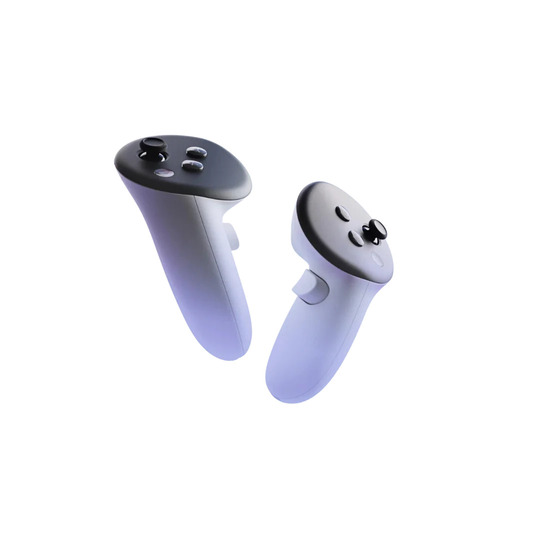
\includegraphics[width=0.35\linewidth]{Background/Quest-3-controllers.png.jpg} % Adjust path and image name
            \captionsetup{justification=centering}

    \caption{VR Controller (\href{https://www.meta.com/de/en/quest/accessories/quest-touch-plus-controller/}{Meta Quest 3})}
  \end{minipage}\hfill
  \begin{minipage}{0.48\textwidth}
    \centering
    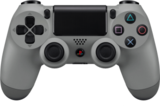
\includegraphics[width=0.4\linewidth]{Background/ps4_controller_png_13_1058.png} % Adjust path and image name
        \captionsetup{justification=centering}

    \caption{ Gamepad (\href{https://www.playstation.com/de-de/accessories/playstation-vr-aim-controller/}{PS Gamepads})}
  \end{minipage}

 
  % Second row
  \begin{minipage}{0.48\textwidth}
    \centering
    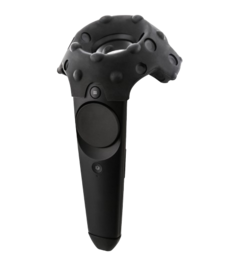
\includegraphics[width=0.3\linewidth]{Background/kisspng-htc-vive-playstation-vr-head-mounted-display-oculu-vive-controller-accessories-5b45845dcff760.0171668615312825258518-removebg-preview.png} % Adjust path and image name
    \caption{Joystick (\href{https://www.vive.com/eu/accessory/controller/}{HTC Vive})}
  \end{minipage}\hfill
  \begin{minipage}{0.48\textwidth}
    \centering
    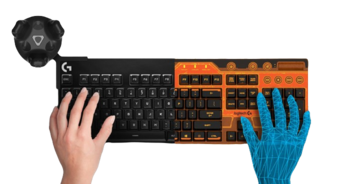
\includegraphics[width=0.48\linewidth]{Background/head-removebg-preview.png} % Adjust path and image name
            \captionsetup{justification=centering}

    \caption{Keyboard (\href{https://www.theverge.com/2017/11/3/16602674/logitech-bridge-sdk-htc-vive-tracker-keyboard}{Logitech})}
  \end{minipage}
\end{figure}
\noindent
Body Gestures, including movements of the head, hands (including fingers), and even blinking, provide alternative interaction methods. For instance, BlinkType and NeckType leverage users’ eye blinks and neck forward and backward movements to select letters , thus offering hands-free interaction\cite{Leng2022}. 

\begin{figure}[h!]
    \centering
    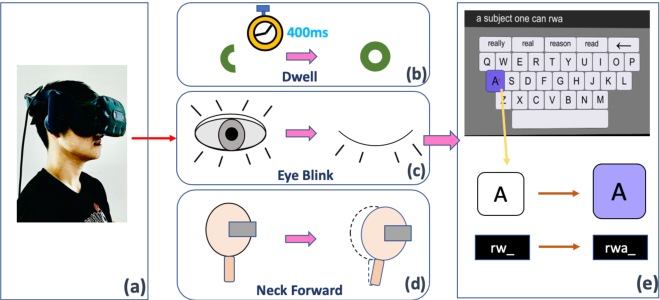
\includegraphics[width=0.7\linewidth]{Background/freehand_Blink.png}
    \caption{An illustration of the text entry with three hands-free techniques in VR \cite{Leng2022}.}
    \label{fig:enter-label}
\end{figure}
\noindent
The realm of haptics also plays a crucial role, with self-referenced haptics focusing on the user's tactile sensations on their own body \cite{hayward2022xr}. Imagine a virtual button placed on the hand of a virtual player; this connection between the user's haptic feedback and their physical presence introduces a new layer of immersion and interaction in \ac{VR} environments.\\ \\ 
Moreover, the Speech-to-Text technique, which converts spoken language into written text, offers a viable alternative when manual entry is impractical or undesired \cite{baljko2006automatic}. The development and refinement of VR text entry techniques have been guided by the need for methods that are both efficient and minimally disruptive, as traditional input devices often do not translate well into \ac{VR} settings \cite{grubert2018text}.\\ \\
The integration of these text entry methods into \ac{VR} applications has opened new avenues for research and development. Studies have shown that the efficiency of text entry systems in\ac{VR} can significantly affect user satisfaction and performance \cite{mcgill2015dovetail}. As \ac{VR} technology continues to evolve, the exploration of more intuitive and natural text entry methods will be crucial. This involves not only technological innovation but also a deep understanding of human-computer interaction principles and user experience design \cite{wickens2015engineering}.\\ \\
Future research should focus on addressing the limitations of current\ac{VR} text entry systems, such as the cognitive load imposed on users and the physical discomfort that may arise from prolonged use. Exploring adaptive systems that can adjust based on the user's input speed and accuracy could provide breakthroughs in usability \cite{hincapie2014metaanalysis}. Additionally, cross-disciplinary studies involving ergonomics, linguistics, and machine learning could lead to the development of more advanced systems that better understand user intent and provide more personalized and context-aware interactions \cite{zhang2017deep}.\\ \\
In conclusion, while significant strides have been made in \ac{VR} text entry technologies, considerable gaps remain in the literature, particularly in terms of comprehensive usability studies and long-term user engagement. Addressing these gaps will not only advance our understanding of \ac{VR} interfaces but also enhance the overall user experience in virtual environments.

\section{Comfortability for virtual typing}
\label{sec:Comfortability for virtual typing} 

In terms of these techniques, long-term comfort is a critical factor when typing on a keyboard within the virtual world. Studies such as those by \cite{dube2019textentry} and \cite{kruger2018text} have highlighted the ergonomic challenges associated with \ac{VR} text entry methods. For instance, head pointing (HP) techniques, where a ray extends from the main camera to facilitate selection, can lead to neck discomfort and dizziness \cite{dudley2019keyboard}. Similarly, Free Hand (FH) and Control Pointing (CP) techniques, while fostering innovation in interaction methods, impose significant physical workloads and can lead to 'gorilla arm fatigue', a term denoting the fatigue resulting from prolonged elevation and use of arms \cite{pseudoHaptics2022}.\\ \\
Moreover, techniques such as Discrete Cursor (DC) and Continuous Cursor (CC) introduce their challenges; both methods may cause texting thumb pain due to repetitive movement \cite{giovannelli2022visual}. An alternative approach involving thumb-to-finger pinch gestures, which offers high spatiotemporal perception and has been reported to increase user satisfaction compared to traditional \ac{VR} keyboards, was explored in \cite{kruger2018text}. This method exemplifies how nuanced gesture control can mitigate some of the physical discomfort associated with more traditional methods.\\ \\
A collaborative study conducted by researchers from the University of Cambridge and the University of Toronto, in partnership with Meta-Reality Labs \cite{leng2022flower}, explored user experiences with different text entry setups in virtual environments. The study found that typing on a virtual keyboard positioned on a physical table led to higher comfort ratings compared to typing in mid-air with either ten or two fingers, showcasing varied comfort levels dependent on the interface used \cite{dudley2019keyboard}. These findings underscore the importance of adaptive interfaces that can dynamically adjust to the user's ergonomic needs and environmental contexts, potentially through the integration of AI-driven systems that learn from user behavior to optimize interface layout and interaction modalities \cite{xu2023haptic}.\\ \\
In addressing the future of \ac{VR} text entry, it is crucial to consider the integration of multimodal feedback systems that combine tactile, visual, and auditory cues to enhance the overall user experience. Such systems could alleviate some of the cognitive and physical strains identified in current technologies by providing more intuitive and natural interaction paradigms \cite{hayward2022xr}. Additionally, advancing haptic technologies could offer more refined and realistic feedback, further enhancing the sense of presence and reducing the disconnect between user actions and system responses \cite{teather2020flik}.\\ \\
Ultimately, the evolution of text entry in virtual reality is contingent upon a multidisciplinary approach that embraces advances in ergonomics, human-computer interaction, and artificial intelligence. By continually refining these systems, we can move closer to creating \ac{VR} environments that are not only effective in terms of task completion but also in promoting user well-being and satisfaction.
\section{Keyboard’s Modernity for virtual typing}
\label{sec: Keyboard’s Modernity for virtual typing} 
Secondly, the modernity of the keyboard in virtual environments is a crucial factor for long-term use. During the study \cite{kruger2018text}, researchers assessed the position and size of the virtual keyboard as essential determinants of usability, emphasizing the keyboard's spatial orientation, including considerations such as left or right-side placement and the optimal distance from the user. The Free Hand (FH) method was noted for its novelty, whereas the Control Pointing (CP) method was found to be most attractive, followed by FH \cite{mcgill2015dovetail}. \\ \\
The type of keyboard consistently used across these studies was Qwerty. However, the shape of the keyboard also impacts usability; two or three-dimensional configurations depend on the application's requirements. For instance, in the study \cite{dudley2019keyboard}, a 2D keyboard was selected because it was fixed to a wooden table and featured keys in a quadratic form, or involved a specific gesture like thumb-to-finger pinch \cite{kruger2018text}. Conversely, another study \cite{pseudoHaptics2022} preferred a 3D keyboard because it floats within the virtual environment, offering a more immersive experience \cite{zhang2017deep}.\\\\
Moreover, the study \cite{teather2020flik} introduced an innovative design called FLIK, where the keyboard keys are arranged in the form of a sphere, deviating from the traditional layout. This spherical arrangement potentially enhances the ergonomic comfort and reduces the cognitive load by aligning more naturally with human hand movements \cite{stanney2019handbook}. Additionally, another study \cite{leng2022flower} pushed the boundaries even further by transforming the keyboard into a flower-shaped configuration while maintaining the order of the QWERTY keys, aiming to combine aesthetic appeal with functional ergonomics \cite{wickens2015engineering}. \\ \\
Each of these innovations reflects ongoing efforts to optimize text entry in virtual environments, highlighting the importance of adaptable interfaces that cater to diverse user needs and preferences \cite{baljko2006automatic, hincapie2014metaanalysis}. As virtual reality technology continues to evolve, the exploration of alternative keyboard layouts and their impacts on user performance and satisfaction will remain a vital area of research \cite{shneiderman2010designing, norman2013design}. \\ \\
The continuous advancement in \ac{VR} technology requires a reevaluation of traditional design principles to include virtual ergonomics and the physiological effects on users, advocating for designs that prevent fatigue and increase user satisfaction \cite{charness2005aging, jacko2009human}.


\section{Keyboard’s Accuracy for virtual typing}
\label{sec: Keyboard’s Accuracy for virtual typing}
When it comes to accuracy, the initial metrics that come into play before pressing a key on the virtual keyboard are key detection and the prevention of typing errors. In a pivotal study \cite{pseudoHaptics2022}, characters are registered when the finger reaches specific distances, precisely 3 cm away from the center of the key (4.5 cm for the Pinch keyboard, as the radius of a sphere was 1.5 cm), and the virtual hands were made semi-transparent to strategically avoid potential collisions. This study proposes a novel technique involving the use of finger-to-thumb as a double-factor confirmation for character entry, enhancing accuracy by confirming intent before final character selection.  \\ \\
Furthermore, the virtual keyboard automatically deactivates all other keys when a collision occurs between the target key and the cursor of the index finger, positioned at the index fingertips to enhance precision during the entry process. This approach is rooted in findings from ergonomic research which suggests that minimizing extraneous movements and providing tactile feedback can significantly reduce entry errors and increase typing speed \cite{mcneill2009gesture, wigdor2011brave}. \\ \\
The integration of spatial and gestural controls as seen in this study aligns with the principles outlined in \cite{norman2013design}, which advocate for natural user interfaces that conform to human motor capabilities and cognitive functions. Additionally, studies such as \cite{zhang2017deep} and \cite{baljko2006automatic} highlight how leveraging deep learning for predictive text input and error correction algorithms can further refine the accuracy of virtual keyboards by anticipating user input and adjusting the interface dynamically. \\ \\
The use of semi-transparent virtual hands and strategic cursor placement also draws upon principles from visual perception psychology, as discussed in \cite{ware2012information}, to reduce visual clutter and enhance the user's focus on target elements, thereby reducing cognitive load and potential input errors. This multidisciplinary approach to interface design, combining HCI, ergonomics, and psychology, is pivotal in developing more intuitive and user-friendly virtual environments \cite{jacko2009human, charness2005aging}.

\section{Haptic Feedback and Visual Feedback in Virtual Environment}

In the realm of feedback within virtual environments, three distinct types are typically identified: haptic, visual, and auditory. In specific studies \cite{teather2020flik, kruger2018text}, haptic feedback primarily involves vibrotactile sensations generated through controllers. This modality not only aids in conveying spatial relationships more effectively than visual and audio feedback alone but also enhances the user’s sense of presence by simulating physical interactions, making these relationships more tangible \cite{hayward2022xr}. \\ \\
While haptic feedback plays a crucial role, visual feedback is also emphasized due to the limited options available for haptic enhancements. In a novel approach, a pseudo-haptic keyboard is introduced with three key features: Protrusion, Hit Effect, and Penetration Blocking \cite{pseudoHaptics2022}. Additionally, a unique pinch keyboard design with bubble-shaped keys is implemented to further enhance user guidance, where the nearest key to the target key is highlighted with a distinct color. Participants in these studies expressed a preference for the Pseudo-haptic and Pinch keyboards, reporting stronger haptic sensation and embodiment compared to a Normal keyboard \cite{zhang2017deep}.\\ \\
Furthermore, another study \cite{teather2020flik} employed a technique called “Big Key,” an algorithm that dynamically adjusts virtual keyboard key sizes based on the likelihood of the next letter in a word. After the initial keystroke, BigKey searches for possible words and scales key sizes according to the frequency of subsequent characters. This approach demonstrated superior performance and high user satisfaction \cite{mcgill2015dovetail}. Conversely, Word Disambiguation, another visual aid technique used in the same study, suggests likely words based on their frequencies as keys are entered, presenting the top three ranked options for efficient word completion. However, this method led to increased frustration and higher mental demand among users \cite{baljko2006automatic}.\\ \\
Each of these feedback mechanisms, whether haptic or visual, plays a pivotal role in shaping the usability and user experience within virtual environments. The integration of advanced feedback techniques, guided by ergonomic and cognitive principles, is crucial for developing interfaces that are both intuitive and effective \cite{jacko2009human, norman2013design}.

\section{Performance for Virtual Typing }
\label{sec: Performance for Virtual Typing}

The performance of virtual typing is not a standalone factor; it is intricately linked to various elements, including the technique employed, the type of feedback (haptic or visual), and the specific use case. Commonly used metrics to measure this performance include Words Per Minute (WPM), Error Rate (ER), Depth of Pressing, Press Duration, and Hand Movements.
Words Per Minute (WPM) is typically defined as the average number of words entered by a user in one minute, with a word usually considered as five characters, including spaces and punctuation:
\begin{equation}
    \text{WPM} = \left( \frac{|T| - 1}{5s} \right) \times 60
  \end{equation} \\ \\
The Error Rate (ER) is the percentage of characters entered incorrectly by the user. ER is calculated by dividing the number of errors by the total number of characters in the text, where \( P \) and \( T \) denote the presented and transcribed text, and MSD is calculated using Levenshtein’s algorithm \cite{levenshteinWiki}:
\begin{equation}
   \text{ER(\%)} = \frac{100 \times MSD(p, T)}{\max(|p|, |T|) }
  \end{equation} \\ \\
Press Duration is the average time that the user's fingers stay on a key after pressing it on the virtual keyboard. This metric can significantly affect the user's feedback, confidence, and satisfaction with \ac{VR} \cite{dube2019textentry}. Additionally, the Depth of Pressing is the average distance that the user's fingers travel in the depth dimension when pressing a key on the virtual keyboard. Depth of pressing can influence the user's fatigue, comfort, and immersion in \ac{VR} \cite{dube2019textentry}.\\ \\
These metrics have been determined through two distinct methods: one involves analyzing the logs generated from keyboard typing, while the other employs a third-party service for calculation. For example, the system in one study \cite{teather2020flik} records the raw input stream. Upon completion, the testbed logs relevant details in a file. In another study \cite{pseudoHaptics2022}, all text entries were conducted through a third-party web application.
\section{Unveiling Omissions}
\label{sec: Unveiling Omissions}

\subsection{Immersion and Realism} 
\label{sec: Immersion and Realism}
Initial studies in the field of \ac{VR} often focused narrowly on haptic feedback limited primarily to simple vibrations, which primarily affected the hand without offering a full spectrum of tactile sensations. This limited approach often led to incomplete sensory experiences, underscoring the need for a more comprehensive exploration of tactile feedback in \ac{VR}. Recent advancements have emphasized the importance of simulating nuanced sensations such as those experienced when grasping or releasing objects. For instance, a study \cite{directionalForce2019} discusses the development of a device that enhances directional sensations in \ac{VR} through mechanical force concentrations using motor rotations. This technology significantly improves the realism of physical interactions, thereby elevating the user's sense of presence and immersion \cite{mcneill2009gesture, stanney2019handbook}.\\ \\
Additionally, the study "Accelerating Skill Acquisition of Two-Handed Drumming using Pneumatic Artificial Muscles" \cite{dasPneumatic} exemplifies the use of advanced haptic systems employing pneumatic artificial muscles to enhance the recall of complex patterns, demonstrating the potential of sophisticated haptic feedback to improve learning and performance in \ac{VR} applications.\\ \\
Moreover, while many studies have focused on distinct text entry methods, there is a notable gap in considering the integration of multimodal inputs, which combine hand gestures with voice commands or elements of auditory and tactile feedback. Such integration is crucial for creating more engaging, convincing, and user-friendly \ac{VR} simulations \cite{wickens2015engineering}. The omission of these synergies could restrict the naturalness and intuitiveness of \ac{VR} text input experiences. Recent research has begun to address these limitations by employing technologies like Word Disambiguation algorithms, which assist in text entry by predicting likely word completions \cite{baljko2006automatic}.\\ \\
Furthermore, while significant attention has been paid to the design of virtual keyboards, there remains a lack of focus on enhancing the virtual hand model to improve interaction during typing tasks. Most studies have maintained a static approach to keyboard orientation in virtual environments, neglecting the potential benefits of a dynamic setup that allows users to navigate and interact more freely within their virtual space. This static approach has often overlooked the significance of environmental textures and other sensory details that could enhance the typing experience and overall interaction quality \cite{spence2008multisensory}.\\ \\
The study "How to Get There When You Are There Already? Defining Presence in Virtual Reality and the Importance of Perceived Realism" \cite{presenceVr2021} further explores the critical role of perceived realism in \ac{VR}. It highlights how users inevitably compare virtual objects with their real-world counterparts and assess their congruence, affecting their overall experience and satisfaction with \ac{VR} technologies \cite{milgram1994taxonomy}.
\subsection{Consistency} 
\label{sec: Consistency}

Consistency in haptic feedback, particularly within virtual environments, has traditionally been limited to static haptic effects—haptic signals that do not change during rendering. This static approach often results in a decrease in user engagement because the repetitive and unchanging nature of the effects fails to mimic the dynamic and varied tactile feedback experienced in real-world interactions \cite{hayward2022xr}. Static haptic feedback can quickly become predictable, reducing the sense of immersion and realism that is crucial for effective virtual environments.
\subsubsection{Challenges of Static Haptic Feedback}
Static haptic feedback systems do not account for changes in user actions or environmental factors, which can lead to a disconnection between the user and the virtual experience. For instance, when interacting with different textures or surfaces in a virtual world, static feedback would fail to provide the nuanced differences users would expect in a real-world scenario \cite{mcgill2015dovetail}. This lack of responsiveness can diminish the perceived quality of the \ac{VR} system and could potentially lead to user dissatisfaction.
\subsubsection{Dynamic Haptic Feedback for Enhanced Engagement}
To address these limitations, more recent studies advocate for dynamic haptic feedback, which adjusts the intensity, pattern, and type of feedback based on the user's interactions and the context within the virtual environment \cite{mcneill2009gesture}. For example, varying the feedback when a user touches different virtual objects—such as changing from a smooth to a textured sensation when moving from a glass surface to sandpaper—can significantly enhance the realism and user engagement.
\subsubsection{Implementations and Technological Advancements}
Several implementations of dynamic haptic feedback have been explored in advanced \ac{VR} systems. Technologies such as haptic suits and gloves equipped with fluid-filled bladders or air pockets that adjust based on the virtual environment have been developed to provide more realistic tactile sensations \cite{stanney2019handbook}. For example, the Teslasuit integrates full-body haptic feedback that can simulate different environmental impacts, from the brush of wind to the impact of a virtual ball.\\ \\
Practical applications of dynamic haptic feedback have been particularly noteworthy in fields such as medical training and remote operations, where the feel of different tissues or materials is crucial. A study involving surgical simulations found that trainees who used \ac{VR} platforms with dynamic haptic feedback performed better and reported a higher level of confidence in their skills compared to those training with static feedback systems \cite{zhang2017deep}.\\ \\
The future of haptic feedback in \ac{VR} is likely to involve a greater integration of AI and machine learning technologies to further refine the responsiveness and adaptability of feedback systems. These advancements could lead to personalized haptic experiences, where the system adjusts not only to general user behavior but also to individual preferences and responses, potentially transforming how users interact with virtual environments \cite{wickens2015engineering}.\\ \\
In conclusion, while static haptic feedback has been a staple in early \ac{VR} applications, the shift towards dynamic, responsive feedback systems represents a significant advancement in the field. By increasing the variability and realism of haptic experiences, \ac{VR} systems can achieve higher levels of user satisfaction and engagement, paving the way for more sophisticated and immersive virtual environments.

\subsection{Skill Transfer and User Experience}
\label{sec:Skill Transfer and User Experience}

Prior research in virtual environments has largely focused on gathering performance data and subjective user feedback, yet often overlooked is the importance of descriptive effects in enhancing user experience. These effects, akin to the MIDI system for musical instruments, represent a method of encoding haptic feedback in a signal-independent manner, which involves detailing only the notes and their 'descriptive' attributes. For example, Apple’s AHAP effect files, part of the CoreHaptics framework, utilize a JSON-based language for describing haptic effects \cite{appleCoreHaptics}. This method allows developers to create expressive and varied haptic sensations without needing a direct motor signal, facilitating richer user interaction. \\ \\ 
Moreover, while metrics like entry speed and error rates are commonly assessed, there is a notable gap in the exploration of other performance indicators that could provide a more holistic view of user experiences. These metrics include the learning curve associated with different text entry methods and the adaptability of users to varying techniques over time. These aspects are critical in understanding the long-term effectiveness and user satisfaction with \ac{VR} interfaces. For example, the accuracy of typing, which is crucial for assessing the effectiveness of text entry methods, can be quantified in several ways:

\begin{equation}
\text{Accuracy in words: } \text{Accuracy} = \left(100\% - \frac{\text{Words with errors} \times 100\%}{\text{Total number of Words}}\right)
\end{equation}

\begin{equation}
\text{Accuracy in characters: } \text{Accuracy} = \left(100\% - \frac{\text{Characters with errors} \times 100\%}{\text{Total number of Characters}}\right)
\end{equation}

\begin{equation}
\text{Accuracy in keystrokes: } \text{Accuracy} = \left(100\% - \frac{\text{Incorrect keystrokes} \times 100\%}{\text{Total number of Keystrokes}}\right)
\end{equation}

\subsubsection{Case Studies and Practical Applications}
Examining case studies where these metrics have been applied reveals their utility in enhancing \ac{VR} training simulations, educational tools, and interactive media. For instance, a \ac{VR} surgical training program that utilized adaptive feedback based on user performance metrics showed that trainees achieved significantly higher accuracy and reduced error rates \cite{vrSurgicalTraining2023}.\\ \\
Another example includes a \ac{VR} language learning application that measured the adaptability of users to different instructional techniques over time, providing valuable insights into how \ac{VR} can be optimized for faster learning curves and better retention rates \cite{vrLanguageLearning2021}.\\ \\
Looking ahead, integrating a broader array of performance metrics into \ac{VR} studies will enhance our understanding and development of user-centric \ac{VR} systems. Future research should also consider the potential of emerging technologies such as artificial intelligence and machine learning to dynamically adapt VR environments to user behaviors, thereby improving the personalization and effectiveness of virtual training environments \cite{aiInVr2023}.\\ \\
In conclusion, while significant strides have been made in capturing performance and subjective data in \ac{VR}, a comprehensive approach that includes descriptive effects and a wider range of performance metrics is essential for the next generation of \ac{VR} applications. Such an approach will not only refine current systems but also pave the way for more sophisticated and immersive user experiences.

\section{Summary}
\label{sec:SummaryBackground}

This chapter provides a comprehensive overview of the varied \ac{VR} text entry methods and their significance in enhancing user interaction and functionality. By employing three key questions—"Why is it being implemented," "How is it being executed," and "What is being utilized"—we have explored the shared intersections and innovative approaches within existing studies. The chapter introduces the primary text entry techniques in \ac{VR}, including the use of physical devices, body gestures, and the Speech-to-Text technique. Each method's role in facilitating effective communication within virtual settings is discussed, highlighting their contributions to reducing cognitive load and increasing typing efficiency.\\ \\
Additionally, the chapter identifies unexplored areas and knowledge gaps in the existing literature, particularly focusing on ergonomic challenges, the integration of adaptive systems, and the need for more comprehensive usability studies. The significance of a multidisciplinary approach involving ergonomics, linguistics, and machine learning is emphasized to foster the development of text entry systems that are both user-friendly and highly functional.\\ \\
In summary, while significant advancements have been made in \ac{VR} text entry technologies, there remains a substantial scope for research, particularly in enhancing the user experience and addressing the limitations of current systems. Future research directions include the exploration of adaptive interfaces and multimodal feedback systems that cater to the ergonomic needs of users and enhance their overall interaction with the virtual environment.


\chapter{Approach}
\label{sec:Approach}

This study aims to address and explore four key objectives, building upon and synthesizing insights gleaned from prior research to significantly enhance the user experience in virtual environments. Our methodology will leverage a comprehensive framework described in the seminal work, "XR Haptics: Implementation \& Design Guidelines" \cite{hayward2022xr}. Each objective is designed to address a distinct aspect of the virtual interaction that contributes to an immersive user experience:

\begin{enumerate}
    \item \textbf{Evolving Haptic Feedback:} We plan to develop dynamic haptic feedback mechanisms during typing on the virtual keyboard. Unlike traditional static haptic effects, our aim is to introduce varying haptic sensations that change contextually based on the user’s interaction patterns and the virtual environment's specific needs. This could include varying the intensity, texture, and feedback pattern in response to typing speed, errors, and keyboard layout changes.
    
    \item \textbf{Enhancing the Virtual Environment:} To elevate the overall user experience, we will refine the environment surrounding the virtual keyboard. This involves integrating more realistic ambient effects, such as lighting changes and subtle background sounds that react to user actions, thereby creating a more engaging and less isolating virtual space.
    
    \item \textbf{Expanding Virtual Hand Capabilities:} Our third objective is to extend the functionality of the virtual hand beyond typing. We aim to enable it to perform more complex and varied tasks, such as gesturing, manipulating virtual objects, and interacting with multiple UI components. This expansion will allow for more natural and versatile user interactions within the virtual environment.
    
    \item \textbf{Implementing Advanced Support Techniques:} Finally, we will employ cutting-edge technologies to enhance the typing process with intelligent features. This includes the integration of predictive text input, adaptive text correction, and personalized haptic feedback based on individual user behavior and preferences. These advanced features are designed to streamline the typing experience, reduce cognitive load, and improve accuracy.
\end{enumerate}
The application of this framework will involve iterative testing and refinement, incorporating user feedback to continuously improve the system's effectiveness and user satisfaction. By addressing these objectives, the study aims to push the boundaries of what is currently possible in VR interactions, setting a new standard for user engagement and system responsiveness in virtual keyboards.


\chapter{Haptics Implementation}
\label{sec:Haptics Implementation}

Building on the fundamental insights provided by "XR Haptics: Implementation and Design Guidelines," this study aims to thoroughly integrate and expand upon the principles of haptic feedback in \ac{VR} environments. By bridging the gap between theory and practice, we seek to optimize user interaction through sophisticated haptic designs that engage users more deeply by mirroring real-world sensations during typing on the keyboard.

\section{Role of Haptics}
\label{sec:RoleOfHaptics}
The role of haptics in \ac{VR} environments is multifaceted, extending beyond simple replication of real-world dynamics to enhancing the virtual experience through strategic feedback modifications. Haptics play a crucial role in reinforcing user actions, providing essential cues that transform the virtual experience from a visual-auditory one into a fully immersive sensory encounter.

\subsection{Realism}
\label{subsec:Realism}
According to "XR Haptics: Implementation Design Guidelines," effective haptic design must prioritize realism to ensure that virtual objects behave as users expect based on their real-world experiences. For the virtual keyboard, this involves simulating not only the typical mechanical response of keys but also incorporating variations such as the tactile feel of different materials or the response from a key with wear over time. Implementing nuanced haptic textures and resistance changes can significantly enhance the perception of realism, making the virtual environment more believable and engaging.

\subsection{Enhanced Immersion through Adaptive Feedback}
\label{subsec:Immersion}
Adaptive haptic feedback, which adjusts in real-time according to user interactions and environmental conditions, is essential for maintaining immersion. This adaptive approach allows the haptic system to introduce feedback that complements changes in the visual and auditory narrative, thus maintaining a consistent and unified user experience. For example, altering haptic feedback based on the virtual environment's ambient conditions—such as changing surface textures or interacting with moving objects—can make the virtual world feel alive and responsive.

\subsection{Skill Transfer and Advanced User Experience}
\label{sec:SkillTransferUserExperience}
Haptic feedback is instrumental in skill transfer from the real world to the \ac{VR} environment. By accurately mimicking the tactile feedback associated with different tasks, users can apply their real-world skills within virtual settings without the typical learning curve associated with new interfaces. For instance, a virtual piano keyboard that replicates the haptic feedback of actual piano keys can aid musicians in performing without looking at the keys, transferring their skills directly into the \ac{VR} domain.

\subsection{Consistency and Customization}
\label{sec:Consistency}
Consistency in haptic feedback helps in reducing the cognitive load on users as they navigate through various virtual scenarios. However, customization plays a pivotal role in catering to diverse user preferences and needs, as highlighted in the "XR Haptics: Implementation and Design Guidelines." By allowing users to adjust the intensity, type, and duration of haptic feedback, the system can accommodate personal sensitivity differences, enhancing comfort and usability.

\section{Haptic Feedback}
\label{sec:HapticFeedback}

After establishing the role of haptic feedback in enhancing virtual interactions, it is crucial to identify the specific types of haptics required for the experiment. As introduced earlier, there are two main categories of haptic feedback: kinesthetic and tactile.

\subsection{Kinesthetic and Tactile Feedback}
\label{subsec:KinestheticTactileFeedback} 
Kinesthetic feedback, often referred to as \ac{FFB}, imparts sensations of force and resistance. This type of feedback divides into two categories: passive and active (or resistive) force feedback. Passive feedback typically functions as a brake, limiting finger or body motion, while active feedback applies direct forces to the user, enhancing the realism of interactions such as lifting or pushing objects within a \ac{VR} environment \cite{hayward2022xr}.\\\\
Conversely, tactile feedback involves sensations directly related to touch, such as vibrations similar to those experienced on a smartphone or contact-spatial feedback, which provides sensations through surface contact without physical interaction. In \ac{VR} environments, tactile feedback is crucial for simulating the realistic click of a keyboard button or the texture of different surfaces.

\subsection{Application in Virtual Keyboards}
\label{subsec:ApplicationInVirtualKeyboards}

In the context of a virtual keyboard, both kinesthetic and tactile feedback play pivotal roles. For tactile interactions, simple non-spatial feedback is often sufficient due to the uniform texture of keyboard keys. However, vibrotactile feedback is essential for delivering nuanced sensations that enhance the user's engagement and perception of reality. For actions that involve more dynamic interaction, such as lifting a virtual keyboard, resistive kinesthetic feedback is utilized to simulate the force and weight of the object.

\subsection{Referential Haptic Feedback}
\label{sec:ReferentialHapticFeedback}

Building on the concept of Referential Haptic Feedback introduced in Section 2.6, our design phase aims to seamlessly integrate this advanced haptic technology into our virtual hand model. This simulation will focus primarily on the user’s hand during the typing process, diverging from traditional methods that simulate multiple aspects simultaneously. By concentrating solely on the hand, we strive to create a more realistic and immersive typing experience, enabling users to interact with the virtual keyboard swiftly and intuitively.

\subsection{Pseudo-Haptics Feedback}
\label{sec:PseudoHapticsFeedback}

Pseudo-haptics involves the integration of visual effects to simulate physical interactions. In our \ac{VR} environment, dynamic changes occur in the shape and color of the keyboard’s keys during typing, accompanied by visual alterations in the keyboard handlers when grasped by the user. Additionally, changes in fingertip coloration help prevent visual penetration, enhancing the realism of interactions.

\subsection{Allocentric and Egocentric Haptics}
\label{sec:AllocentricEgocentricHaptics}

The haptic feedback in our \ac{VR} environment operates within a three-dimensional framework and is categorized into two distinct types: Allocentric and Egocentric. Allocentric haptics depict spatial relationships among objects within the environment, enhancing the user's external spatial awareness. Egocentric haptics, conversely, illustrate the spatial relationships between the user and immediate objects, such as the virtual keyboard, ensuring that feedback is directly related to the user's interactions.

\subsection{Multimodal Integration}
\label{sec:MultimodalIntegration}

The integration of multiple sensory modalities is crucial for creating compelling and immersive simulations. Our approach uses the "reinforce" method, where haptic feedback is synchronized with auditory and visual elements to enrich the overall experience. This multimodal integration reinforces the tactile sensations with corresponding audio-visual cues, enhancing the user's engagement and satisfaction while interacting with the virtual keyboard.
\section{Summary}
\label{sec:Summary}

This chapter on Haptics Implementation has focused on enhancing the realism and immersion of \ac{VR} environments through sophisticated haptic feedback. Building on principles from the "XR Haptics: Implementation and Design Guidelines," we discussed the role of haptics in creating a fully immersive sensory experience, emphasizing realism, adaptive feedback, and user customization.\\ \\
Specific types of haptic feedback, including kinesthetic and tactile feedback, were identified as critical for simulating realistic interactions within \ac{VR} environments, particularly in applications like virtual keyboards. The chapter also introduced innovative haptic technologies such as Referential and Pseudo-Haptics Feedback, and discussed the importance of multimodal integration in reinforcing user engagement and satisfaction. Overall, the chapter aims to bridge the gap between theoretical insights and practical applications in haptic design to optimize user interaction in virtual settings.

\chapter{Hardware and Software Selection}
\label{sec:HardwareSoftwareSelection}

Building upon insights from the previous chapters and the integral role of haptic feedback in enhancing user experience, this section delineates the specific hardware components and software solutions capable of delivering sophisticated haptic feedback for keyboard typing in virtual environments.

\section{Head-mounted Devices}
\label{sec:HeadMountedDevices}

In our investigation, the Meta Quest 3 is selected as the primary head-mounted display (HMD) due to its superior features when compared to its predecessors and competitors. This decision follows a comprehensive analysis of its capabilities in contrast to the HTC Vive and Oculus Rift.

\begin{itemize}
    \item \textbf{Meta Quest 3} offers a high-resolution LCD (2064x2208 per eye), a 120Hz refresh rate, and advanced tracking capabilities including 6 degrees of freedom (DoF) inside-out tracking via 4 integrated cameras and a depth sensor. It supports hand tracking and includes two 6DoF Meta Quest Touch Plus Controllers, providing robust connectivity options such as WiFi streaming, WiFi 6E, and Bluetooth.
    
    \item \textbf{HTC Vive}, on the other hand, features an OLED display with a resolution of 1080x1200 per eye and a 90Hz refresh rate. It employs a marker-based tracking system and includes two 6DoF HTC Vive controllers but lacks hand tracking, WiFi, and Bluetooth.
    
    \item \textbf{Oculus Rift} provides an AMOLED display with a resolution of 1080x1200 per eye and a 90Hz refresh rate. It uses an outside-in tracking system and includes two first-generation 6DoF Oculus Touch controllers but does not support hand tracking, WiFi, or Bluetooth.
\end{itemize}
Given these specifications, Meta Quest 3 is chosen for its cutting-edge display quality, superior tracking, and enhanced connectivity, making it the most suitable option for our experiments.

\section{Haptic Sensations and Devices}
\label{sec:HapticSensationsDevices}

The role of haptic devices in virtual reality is to bridge the gap between the real and virtual worlds by transmitting tactile sensations. A company named SynTouch has developed a product known as the SynTouch-Toccare Haptics Measurement System, capable of quantifying 15 haptic dimensions of any material, thus replicating human touch perception. This technology is pivotal in providing a nuanced understanding of material textures and interactions within the virtual environment.
\begin{figure}[ht]
  \centering
  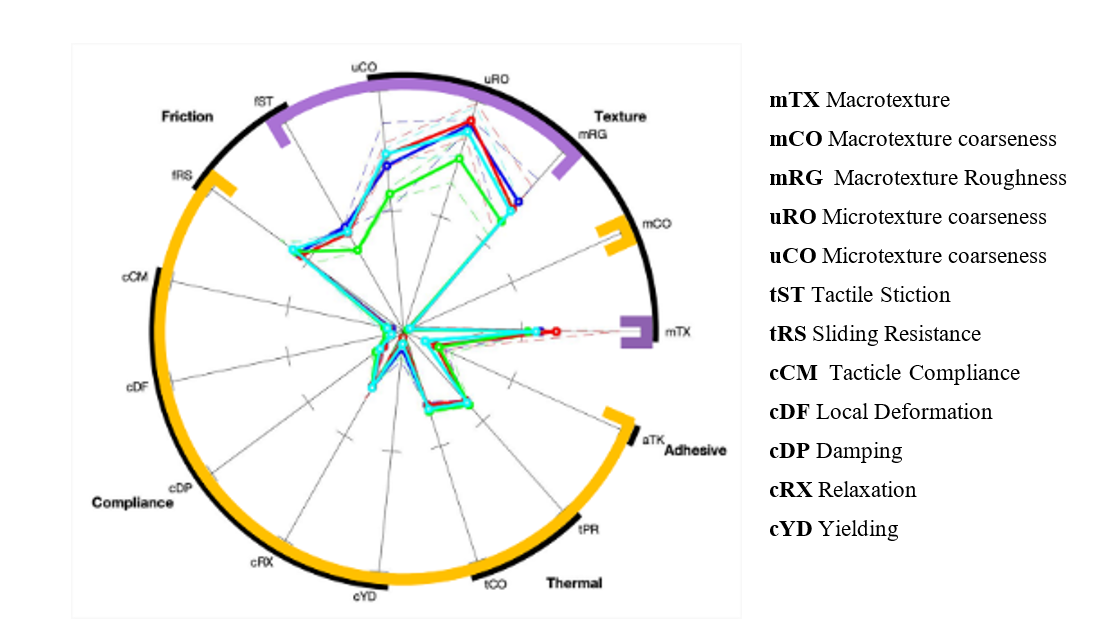
\includegraphics[width=0.8\textwidth]{Development/senstations.PNG}
  \caption{SynTouch's 15-Dimensional Sensations \cite{quantifying_touch}}
  \label{fig:sensations}
\end{figure}

\subsection{Advanced Haptic Gloves}
\label{subsec:AdvancedHapticGloves}

For the experimental setup, we propose using the SenseGlove Nova, renowned for its advanced haptic feedback capabilities and innovative design. The SenseGlove Nova offers a range of features that enhance the realism and immersion of virtual reality interactions:

\begin{figure}[ht]
\centering
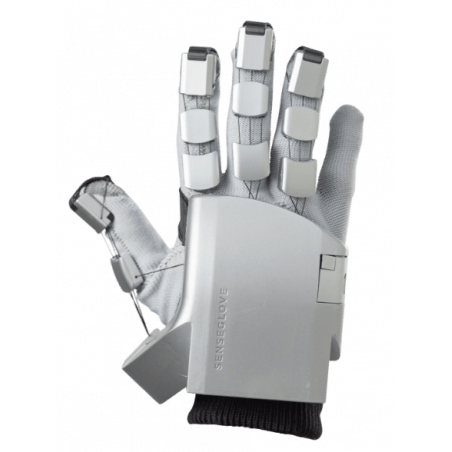
\includegraphics[width=0.35\textwidth]{Development/sense-glove-nova-set.jpg}
\caption{The Sense Glove Nova \cite{senseglove_nova}}
\label{fig: The Sense Glove Nova}
\end{figure}

\begin{itemize}
\item \textbf{Force Feedback:} Each glove is equipped with high-precision brakes that deliver up to 20N of force on each finger. This feature enables users to feel the weight and resistance of virtual objects, ranging from heavy tools to delicate items, providing a more authentic interaction experience \cite{senseglove_nova}.
\item \textbf{Vibrotactile Feedback:} The SenseGlove Nova incorporates vibrotactile actuators that generate realistic sensations such as button clicks, vibrations, and impacts. This feedback significantly enhances the user's sense of touch and engagement with virtual environments \cite{vibrotactile_feedback}.

\item \textbf{Sensor-Based Tracking:} The gloves utilize multiple high-accuracy sensors to capture the movements of the thumb and fingers. This precise tracking is crucial for accurate hand representation in virtual reality, ensuring that user actions are mirrored accurately within the virtual space \cite{sensor_tracking}.
\end{itemize}
\noindent
The SenseGlove Nova's combination of force feedback, vibrotactile feedback, and precise tracking makes it an ideal choice for applications requiring detailed and nuanced hand interactions. Its advanced technology supports a wide range of virtual reality applications, from training simulations to interactive gaming, by providing users with a tactile experience that closely mimics real-world interactions.\\ \\
The use of SenseGlove Nova in our experimental setup is expected to significantly enhance the user experience by providing realistic and responsive haptic feedback. This technology not only improves the immersion but also aids in tasks requiring fine motor skills and detailed manipulation of virtual objects, making it a valuable tool for our virtual reality system \cite{advanced_haptic_gloves_review}.

\section{Virtual Environment Development with Unity}
\label{subsec:VirtualEnvironmentDevelopmentWithUnity}

Unity will be utilized for developing the virtual environment in which the virtual keyboard will be used. The advantages of using Unity include:
\begin{itemize}
\item \textbf{Real-Time Rendering:} Unity's powerful real-time rendering capabilities ensure smooth and immersive visuals, essential for creating a realistic virtual environment.
\item \textbf{Cross-Platform Support:} Unity supports multiple platforms, allowing the virtual environment to be accessible on various devices, from VR headsets to mobile devices and PCs.
\item \textbf{Extensive Asset Store:} Unity's Asset Store provides a vast array of pre-made assets, scripts, and plugins that can accelerate development and add rich features to the environment.
\item \textbf{Robust Developer Community:} A large and active community of developers means extensive support, tutorials, and forums for problem-solving and learning.
\item \textbf{Seamless Integration with Other Tools:} Unity can easily integrate with other development tools and software, facilitating a cohesive and efficient development process.
\end{itemize}
Using Unity ensures that our virtual environment will be engaging, versatile, and accessible, providing users with a seamless and immersive experience while interacting with the virtual keyboard.


\section{Keyboard Design with Blender}
\label{subsec:KeyboardDesignWithBlender}

For the design and modeling of the virtual keyboard, we will use Blender, a powerful and versatile 3D modeling software. Blender is chosen for several reasons:
\begin{itemize}
\item \textbf{Comprehensive Toolset:} Blender offers an extensive range of tools for modeling, sculpting, texturing, and rendering, making it an all-in-one solution for creating detailed and high-quality 3D models.
\item \textbf{Open Source and Free:} Blender is open-source software, which means it is free to use. This allows us to allocate resources to other aspects of the project while still utilizing professional-grade software.
\item \textbf{Community Support and Documentation:} Blender has a large, active community and extensive documentation, providing ample resources for troubleshooting and learning advanced techniques.
\item \textbf{Integration Capabilities:} Blender supports various file formats and can be integrated with other software tools used in our project, ensuring a smooth workflow.
\end{itemize}
Using Blender allows us to create a highly detailed and customizable virtual keyboard, enhancing the user's interaction experience by providing a visually appealing and functional design.

\section{Integration With Meta Quest 3}
\label{subsec:IntegrationWithMetaQuest3}

The integration of SenseGlove Nova with the Meta Quest 3 is facilitated through the SenseGlove Nova SDK \cite{senseglove_sdk} . Connections can be established via Bluetooth or by directly linking the glove's controller transform object into the virtual environment setup. This integration allows for precise control over force feedback and tactile sensations, ensuring a rich and immersive user experience.





\section{Assisting and Guiding}
\label{sec:AssistingGuiding}

In addition to enhancing the surrounding area of the virtual keyboard to assist users during typing by providing directions and guidelines, we will integrate advanced language understanding features through a third-party service called ChatGPT. This integration aims to improve the structure and content of entered text by offering sentence and word suggestions \cite{openai, ioshacker}. Users will be able to select the most suitable suggestion for their attention, thus elevating the overall typing experience. ChatGPT, trained on a diverse range of internet text, possesses advanced language understanding capabilities, enabling it to generate human-like text based on provided context \cite{openai}. This unique attribute makes it an ideal tool for suggesting contextually relevant and grammatically correct words or sentences, surpassing the capabilities of simple auto-correct systems. Unlike traditional auto-correct systems that focus solely on the last word typed, ChatGPT provides contextual suggestions by considering the overall context of the sentence \cite{yellow, online-tech}. This approach results in more accurate and helpful suggestions, contributing to an improved user experience. \\ \\
The integration of ChatGPT goes beyond correcting typos; it enriches the typing experience by allowing users to explore different ways to express their thoughts with the assistance of versatile suggestions. This not only enhances efficiency but also adds an element of enjoyment to the typing process \cite{ioshacker}. Furthermore, ChatGPT's continuous learning capability as a machine learning model means that it can improve over time. The more it is utilized, the better it becomes at providing relevant suggestions, ensuring a dynamic and evolving tool for users. In terms of versatility, ChatGPT can be seamlessly adapted to various applications, making it a valuable tool in diverse scenarios beyond typing assistance. Its versatility extends its utility across different domains, showcasing its potential as a multifaceted solution \cite{openai}.



\section{Summary}
\label{sec:Summary}

Selecting appropriate hardware and software is crucial for achieving a high-fidelity virtual experience. The chosen devices support advanced delivery of haptic feedback and ensure a seamless, intuitive user experience. By integrating these technologies, we aim to create a virtual typing interface that closely mimics real-world interactions, thereby enhancing realism and effectiveness in the virtual environment.

\chapter{Conception}
\label{sec:Conception}

Building upon the insights from previous chapters regarding the pivotal role of haptic feedback, this chapter transitions from theoretical discussions to the practical implementation phase of our study. We have explored the rationale for incorporating haptic feedback, its intended applications, and the specific tools planned for use. Now, we move forward to actualize these concepts, beginning with a general use case diagram to visually represent system interactions. Following this, we will examine the visual aspects of our 3D interface and conclude by elucidating the underlying mechanisms that support our proposed solutions. This comprehensive approach ensures that our transition into the implementation phase is well-founded, aiming to enhance user experience through detailed planning and thoughtful design.

\section{General Use Case}
\label{sec:GeneralUseCase}

This section introduces the General Use Case diagram, which serves as a crucial visual tool depicting the dynamic interactions between users and the core functionalities planned for our \ac{VR} environment experiment. This diagram provides a comprehensive overview of the various scenarios and interactions that users may encounter, elucidating how they engage with the key features incorporated into the system.

\begin{figure}[ht]
\centering
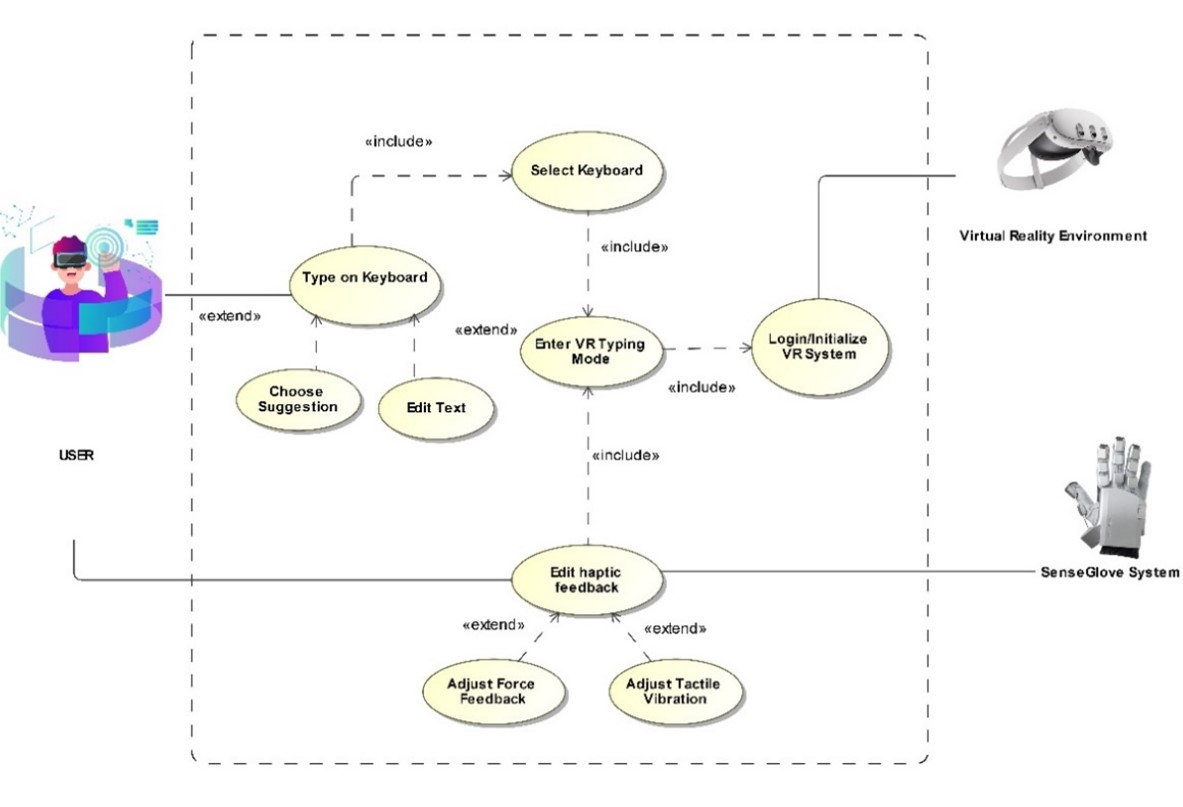
\includegraphics[width=0.8\textwidth]{Development/Picture1.jpg}
\caption{General Use Case Diagram for our experiment}
\label{fig:GeneralUseCaseDiagram} 
\end{figure}
\noindent Accompanying the diagram, Table~\ref{tab:GeneralUseCases} details the specific use cases, providing a structured description of each scenario within the \ac{VR} environment. This table categorizes user interactions, from initiation through various interaction phases, to modifications in settings, highlighting the system's response to each action.

\begin{table}[htbp]
\centering
\begin{tabular}{|p{4cm}|p{8cm}|}
\hline
\textbf{Use Case} & \textbf{Description} \\
\hline
Login/Initialize \ac{VR} System & To initiate the activity, the user is required to verify their identity, ensuring secure access to the virtual environment. \\
\hline
Enter \ac{VR} Typing Mode & Following successful login, the user transitions seamlessly into the immersive virtual typing environment. \\
\hline
Select Keyboard & The user selects the keyboard layout and settings to start typing, choosing from various available configurations. \\
\hline
Type on Keyboard & Interaction begins as the user types on the virtual keyboard, engaging with digital content creation. \\
\hline
Choose Suggestions & Users can select from contextually relevant suggestions provided by the system while typing, enhancing typing efficiency and accuracy. \\
\hline
Edit Text & Users have the flexibility to edit text at any point, with options to add, delete, or rearrange content as needed. \\
\hline
Edit Haptic Feedback & Users can enter a mode to customize the haptic feedback settings according to their personal preference. \\
\hline
Adjust \ac{FFB} & Users can fine-tune the intensity of \ac{FFB} to match their desired level of tactile response. \\
\hline
Adjust Tactile Vibration & The intensity of tactile vibrations can be adjusted, allowing users to tailor the haptic experience to their comfort and liking. \\
\hline
\end{tabular}
\caption{Descriptions of General Use Cases}
\label{tab:GeneralUseCases}
\end{table} 
\noindent Each use case outlines critical interactions within the system, ensuring that user needs and preferences are meticulously catered to, from system initiation to detailed personalization of the typing experience. This structured approach not only enhances user satisfaction but also fosters an intuitive and engaging interaction environment.
\clearpage
\section{Network Diagram}
\label{sec:NetworkDiagram}

Following the identification of the primary use cases, we now focus on examining the intercommunication among the key hardware components of our \ac{VR} environment setup. The network diagram presented in Figure~\ref{fig:NetworkDiagram} offers a detailed visual representation of the interaction among these components, which include advanced haptic gloves, the Execution Environment, the local subnet, and the \ac{HMD}. This diagram is essential for understanding how data flows within our system and how components are interconnected to support seamless user interactions.

\begin{figure}[htbp]
\centering
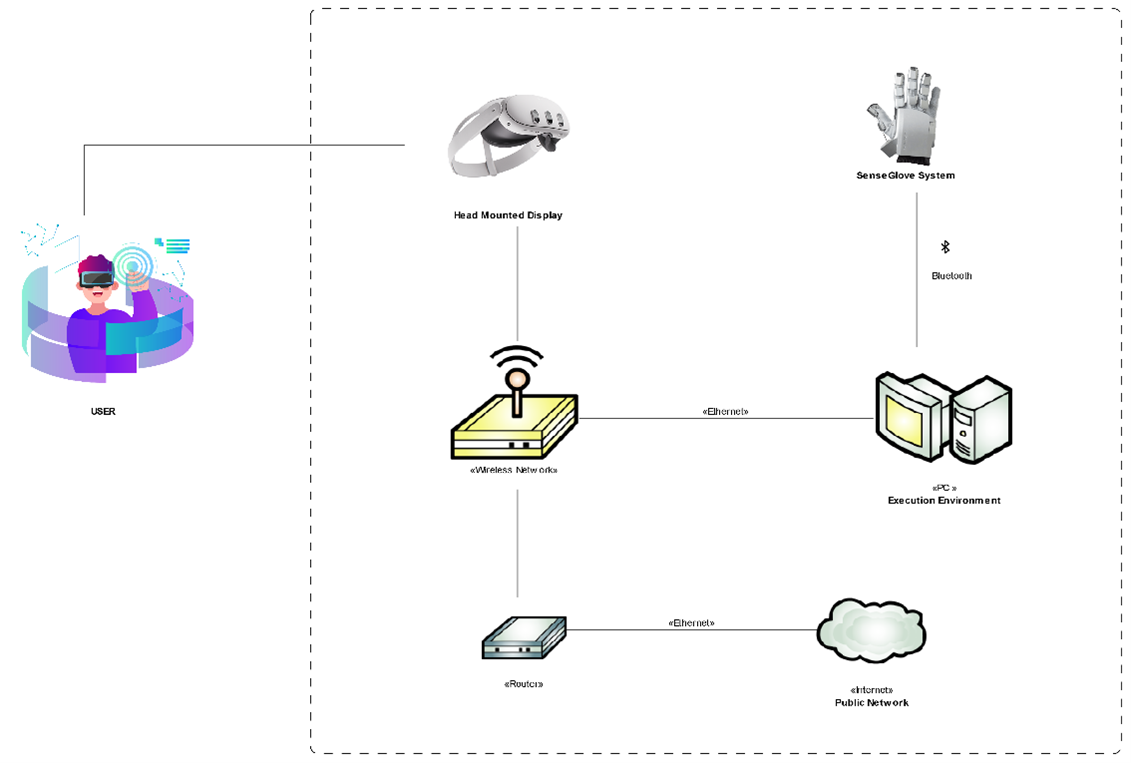
\includegraphics[width=1\textwidth]{Development/networkDiagram.png}
    \captionsetup{justification=centering}

\caption{Network Diagram showing the interconnectivity of system components.}
\label{fig:NetworkDiagram}
\end{figure}

\clearpage

\begin{table}[htbp]
\centering
\begin{tabular}{|p{3cm}|p{9cm}|}
\hline
\textbf{Hardware} & \textbf{Description} \\
\hline
SenseGlove Nova & The SenseGlove Nova transmits sensory data to the Execution Environment via Bluetooth. It can also establish a direct connection to the \ac{HMD} when required. \\
\hline
Wireless Network & Communication between the \ac{HMD} and the Execution Environment is facilitated through Air Link, a high-performance wireless connection that supports real-time data exchange. \\
\hline
Execution Environment & All scenario executions occur locally within this environment, employing Bluetooth as the primary communication protocol to ensure rapid and secure data transfer. \\
\hline
Router & The router plays a pivotal role in managing communications between the \ac{HMD}, Execution Environment, and the public internet, ensuring robust and reliable connectivity. \\
\hline
Head-Mounted Device (\ac{HMD}) & The \ac{HMD} communicates with the Execution Environment using the TCP protocol to facilitate seamless access and synchronization with the public internet. \\
\hline
\end{tabular}
\caption{Descriptions of the Network Diagram Components}
\label{tab:NetworkDiagram}
\end{table}
\noindent
This network setup is designed to optimize the flow of information and control signals across different components of the system, ensuring that the \ac{VR} environment operates smoothly and efficiently. The integration of these components via robust communication protocols and network connections is critical for delivering a responsive and immersive user experience, thereby enhancing both the realism and functionality of the virtual environment.

\section{Virtual Keyboard’s Conception}
\label{sec:Virtual Keyboard Conception}
While smartphones have become the most used hardware in the market, surpassing other devices \cite{Laricchia2024}, they still rely on fundamental components common to many hardware devices. For instance, consider the conventional structure of a keyboard, which is an integral part of many devices, not just computers but also smartphones in the form of digital keyboards.\\ \\
The keyboard comprises two primary components: the keys and the substrate. The substrate is a planar surface responsible for housing and supporting the keys. In the context of a smartphone, the ‘keys’ are the touch-responsive elements displayed on the screen, and the ‘substrate’ is the underlying software framework that captures and interprets key presses \cite{Staff2022}. Given user familiarity with the established paradigm of smartphone keyboard architecture, the design of the keyboard will conform to this norm. Consequently, emphasis will primarily be directed toward the clarification and optimization of the aforementioned two components.\\ \\
Hence, our goal is to replicate the smartphone keyboard in a \ac{VR} environment. The following sections delve into the intricacies of the keyboard design slated for use in the forthcoming immersive experience.

\subsection{Conceptualization of the Board}

To make a virtual keyboard look and act real, attention to detail is crucial. By replicating as many features as possible, the virtual version can seem more genuine. A study \cite{Ying2021} investigated the impact of QWERTY and T9 \cite{T9} input methods on smartphone text input across various sizes (4.7 inches, 5 inches, and 5.5 inches). Findings indicate that QWERTY is more effective for two-thumb input, and T9 for one-thumb input, with two-thumb entry providing an overall superior user experience. Optimal performance was observed with QWERTY and T9 on a 5-inch smartphone and QWERTY on a 5.5-inch smartphone.

\begin{figure}[h!]
    \centering
    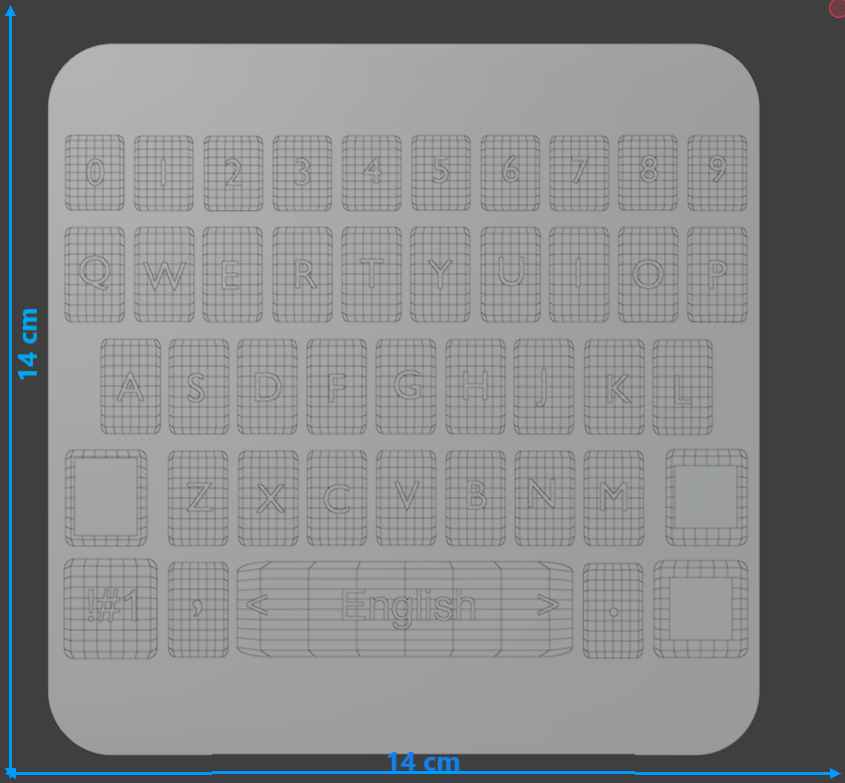
\includegraphics[width=0.7\linewidth]{Development/keyboard_size.png}
    \caption{Schematic representation of the virtual keyboard layout used for testing QWERTY input methods, displayed in Blender viewport shading (Solid Display).}
    \label{fig:keyboard_sin}
\end{figure}
\noindent
In addition to keyboard size, the most commonly used colors for smartphone keyboards are black, gray, and white. This is supported by the popularity of black as a phone color and the prevalence of these colors in top Android keyboards like Fleksy, Gboard, and SwiftKey \cite{Muelaner2023}. These colors are likely chosen for their neutrality, which allows them to blend well with various phone themes and user preferences.\\ \\

\begin{figure}[h!]
    \centering
    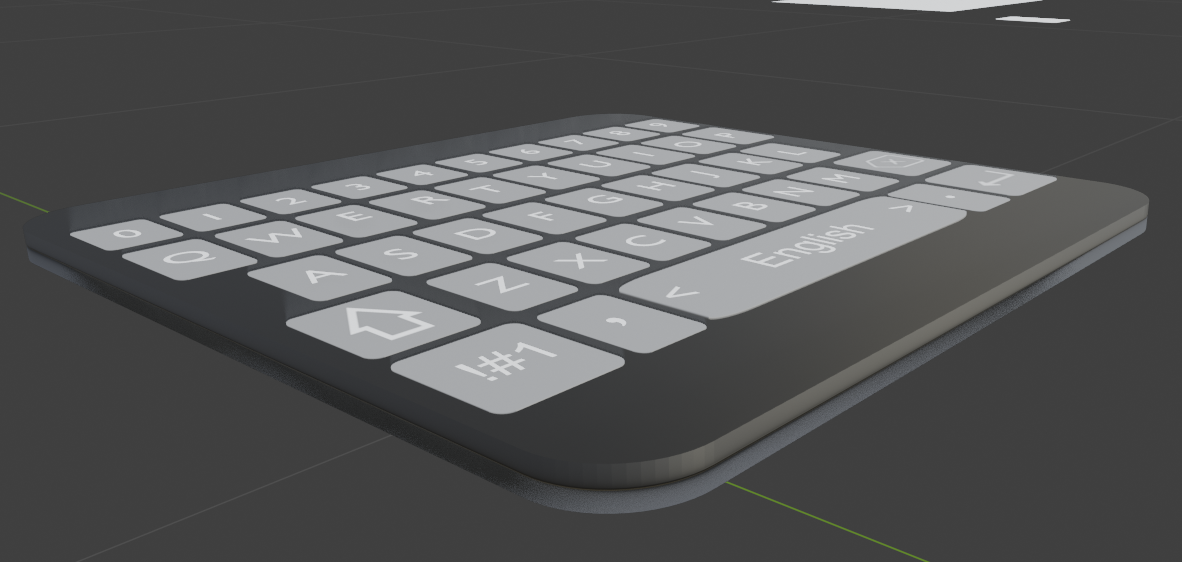
\includegraphics[width=0.7\linewidth]{Development/keybordViewPort.PNG}
    \caption{Schematic representation of the virtual keyboard layout used for testing QWERTY input methods, displayed in Blender viewport shading (Material Display). }
    \label{fig:keyboard_sin}
\end{figure} \noindent
To enhance the portability of our keyboard, integrating hand support is imperative, aiming to emulate the familiar grip of a smartphone. This augmentation contributes to a heightened sense of realism and immersion in \ac{VR} experiences, allowing users to interact with the keyboard in a manner akin to physical settings, even while wearing gloves. Moreover, ensuring universal comfort necessitates careful consideration of users' hand dimensions. According to the National Aeronautics and Space Administration (NASA), the average hand length for males is 7.6 inches, with a breadth of 3.5 inches and a circumference of 8.6 inches. Correspondingly, for females, these dimensions are 6.8 inches, 3.1 inches, and 7.0 inches, respectively. Incorporating this data allows us to ensure that the thumb can comfortably reach the edge of the keyboard when the user enters the typing mode, ensuring a user-friendly and universally comfortable device \cite{nasa_anthropometry,nasa_hand_dimensions,nasa_performance}.

\subsection{Key Conception for the Keyboard}

In our pursuit to optimize the \ac{VR} keyboard and replicate the efficiency of physical typing, we propose a distinctive proportion mechanism aimed at minimizing typing errors. This mechanism operates by identifying the key with the largest contact area with the virtual finger. To streamline this process, we advocate for the division of each virtual key into multiple sections.\\ \\
To implement this division, we suggest employing a grid-based method. Each virtual key's surface is subdivided into cells of equal size, forming a grid. The dimensions of this grid are determined by the average size of the virtual fingertip and the size of the virtual key. For instance, if both the virtual key and the average virtual fingertip measure 10 mm x 10 mm, we could opt for a 3x3 or 8x10 grid configuration. \\ \\

\begin{figure}[h!]
    \centering
    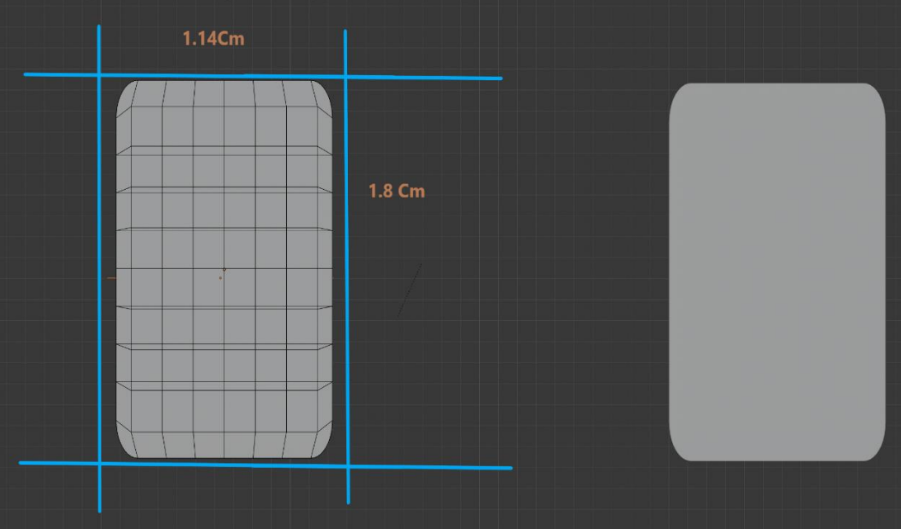
\includegraphics[width=1\linewidth]{Development/keyboard_image2.PNG}
    \caption{Schematic representation of the virtual key layout used for testing QW-
ERTY input methods, displayed in Blender viewport shading (Solid Display)}
    \label{fig:enter-label}
\end{figure}
\noindent 
The subsequent step involves scrutinizing each cell within the grid to assess the degree of contact with the virtual finger. This assessment is facilitated by incorporating a texture on the surface of the thumb finger of the virtual hand model, as provided by the SenseGlove Nova SDK. \\ \\
To enhance the user experience, we propose integrating an animation feature. The shape of the virtual key during interaction will mimic the shape it takes when pressed on a smartphone. A pop-up animation will accompany this interaction, visually indicating the pressed key. When designing virtual keyboards, particularly the size of the keys, it's essential to balance ergonomics with functionality to enhance user experience and performance. Research indicates that key size can significantly affect typing speed, accuracy, and overall comfort. According to a study \cite{Kim2013}, key sizes on touch screen virtual keyboards influence productivity, usability, and typing biomechanics, suggesting that virtual keyboards with a key size less than 16 mm may slow typing speed and increase wrist extension, highlighting the importance of optimizing key size for user comfort and efficiency. Another study \cite{Productivity2014} proved that virtual keyboards with key sizes smaller than recommended (18 to 20 mm for notebook and desktop keyboards) can lead to slower typing speeds, higher muscle activity, and greater wrist extension, indicating potential discomfort and reduced productivity. Keyboards with 13x13 mm keys, for example, resulted in a 15\% slower typing speed and higher static shoulder muscle activity compared to larger key sizes.\\ \\
For a \ac{VR} smartphone keyboard, choosing the right texture for the keys is essential to enhance realism and user experience. The texture should provide visual cues that simulate the feel of a real keyboard. Research in human-computer interaction (HCI) \cite{Fitts2004} has shown that reducing glare and reflections on surfaces can improve visibility and reduce eye strain. A Dark texture on the \ac{VR} keyboard keys can help achieve these goals, making it easier for users to see and interact with the keyboard.

\section{Dynamic Virtual keyboard Interactions}

\subsection{Key Press Animation Feedback}
For key press animation, the goal is to provide immediate feedback to the user, indicating that their input has been recognized. This type of animation falls under the category of micro-interactions. These animations are crucial in making interactions feel more tangible and responsive \cite{Hannah2021}. Therefore, a 0.2-second animation at 30 frames per second, resulting in 6 frames, would be consistent with these principles, offering a quick and responsive feedback loop that enhances the user experience without overwhelming the user with unnecessary motion or delay.\\ \\
In our project, the scale values were adjusted during the animation. The X and Y components were each increased by approximately 11\%, while the Z component was increased by approximately 4\%. These adjustments were calculated to provide a noticeable yet subtle feedback effect, aligning with the principles of effective micro-interactions and ensuring a smooth, responsive user experience. We found that this scale percentage is the optimal size to avoid key collision during scaling, ensuring that the keys remain distinct and accessible during the animation. 
 \begin{figure}[h!]
\centering
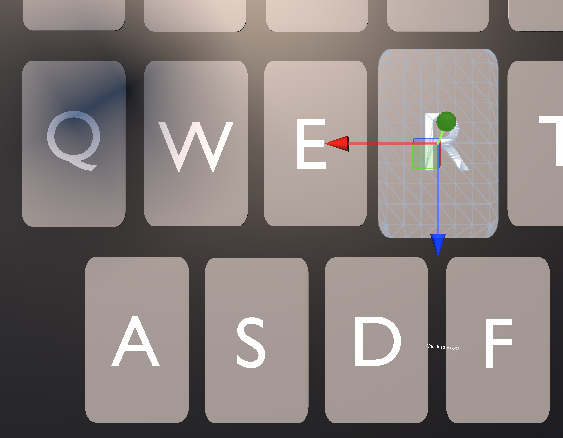
\includegraphics[width=0.8\textwidth]{Development/key_AfterAnimation.PNG} 
\caption{Key Appearance After Animation}
\end{figure}

\noindent
\\\\                
\noindent
\\\\  \noindent
\\\\  \noindent
\\\\  \noindent


\subsection{Hover Effect Implementation}

In virtual reality (VR) environments, providing immediate visual feedback to users significantly enhances their interaction experience, improving both accuracy and comfort. One critical aspect of this feedback mechanism is the hover effect, which visually highlights key parts as users move their fingers over them. This section explains the logic behind the hover effect implementation in the VR keyboard, including the dynamic color changes of the key parts.

\subsubsection{Detection of Hovered Key Parts}

The hover effect is implemented by continuously monitoring the position of the user's thumb in the VR environment. A virtual bounding box is defined around the thumb, and this box is used to detect any interaction with the virtual keyboard key parts.

\subsubsection{Raycasting Technique}

To determine which key parts are being hovered over, a technique called raycasting is used. This involves projecting a virtual box around the thumb's position and checking for intersections with the key parts on the virtual keyboard. The system identifies which key parts are within this box, indicating that they are being hovered over by the user's thumb.

\subsubsection{Visual Feedback Mechanism}

Once a key part is detected as being hovered over, the system provides immediate visual feedback by changing the appearance of the key part. This visual change primarily involves altering the color of the key part. The color transition is determined based on a predefined start color and end color, and the specific weight assigned to each key part. The weight represents the degree of interaction or importance of the key part, allowing for a smooth gradient transition between the start and end colors \cite{douglas1999impact} .

\subsubsection{Handling Multiple Key Parts}

The system keeps track of the key parts that were previously hovered over. If the thumb moves away from a key part, the visual feedback for that key part is reset to its original state. This ensures that only the currently hovered key parts are visually highlighted, providing real-time feedback as the user moves their thumb across the virtual keyboard.

\subsubsection{Interaction States}

The hover effect is closely integrated with the overall interaction states of the virtual keyboard. When no key part is actively being pressed, the system focuses on detecting and highlighting the key parts being hovered over. If a key part is pressed, the hover detection is temporarily paused to prevent conflicts between hover and press feedback.

\subsubsection{Dynamic Color Adjustment}

The system dynamically adjusts the color of the key parts based on the user's actions. When a key part is hovered over, its color changes according to a calculated weight. The weight determines the blend between the start and end colors, using a linear interpolation technique to create a smooth transition. This provides immediate and clear visual feedback, enhancing the user's interaction experience. When the thumb moves away, the key part's color is reset to its original state, ensuring that the visual feedback accurately represents the current interaction state \cite{bolt1980put}.

\subsubsection{User Experience Enhancement}

By providing immediate and clear visual feedback through the hover effect, including dynamic color changes, the system enhances the user's typing experience in the VR environment. Users can easily see which key parts they are about to press, reducing errors and increasing typing efficiency. This real-time feedback is crucial for creating a more intuitive and engaging virtual interaction \cite{norman2013design}.

\subsection{Key Press Sound Feedback} 

In our project, we aimed to generate unique audio feedback for each key press on a virtual keyboard. The process involved modifying the pitch of a base click sound to create distinct auditory signals for each key, ensuring that each key press has a unique sound effect. This approach enhances the user experience by providing clear and immediate auditory feedback, aligning with the principles of effective micro-interactions. We utilized the \texttt{pydub} library for audio processing \cite{pydub}, which was responsible for loading, modifying, and exporting audio files.

\subsubsection*{1. Pitch Modification}

Pitch modification refers to changing the frequency of an audio signal to alter its pitch without changing its duration \cite{smith1999}. This is a crucial technique in audio processing used to create variations in sound.\\ \\
\noindent
The core principle behind generating unique sounds for each key is pitch shifting. Pitch shifting involves changing the frequency of an audio signal without altering its duration. Mathematically, this is achieved by altering the sample rate of the audio signal.
The relationship between the original frequency (\( f \)) and the modified frequency (\( f' \)) when shifting the pitch by \( s \) semitones is given by:
\begin{equation}
f' = f \cdot 2^{\frac{s}{12}}
\end{equation}


where:
\begin{itemize}
  \item \( f \) is the original frequency,
  \item \( f' \) is the new frequency after pitch shifting,
  \item \( s \) is the number of semitones by which the pitch is shifted.
\end{itemize}
\begin{figure}[h!]
    \centering
    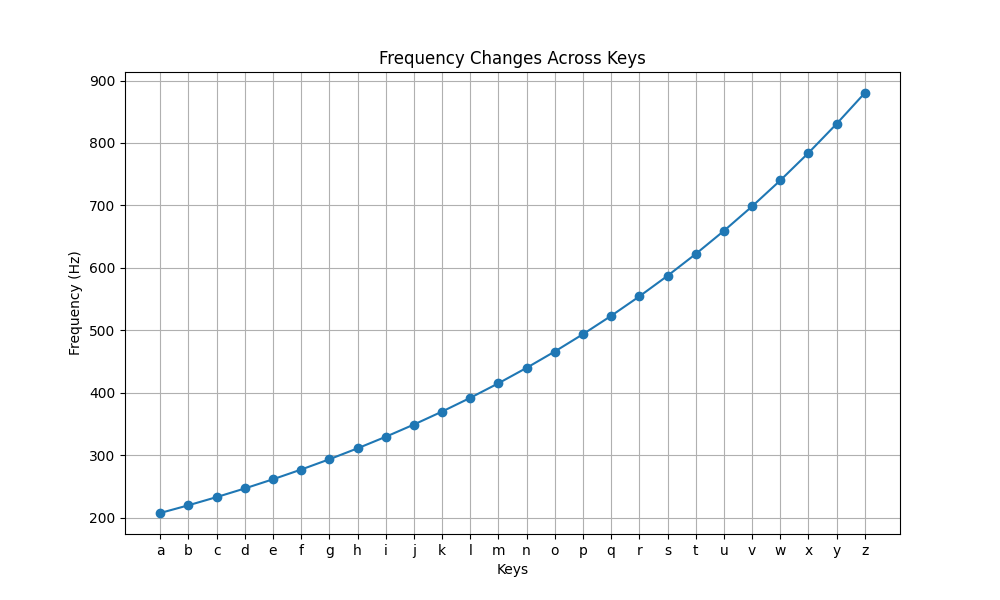
\includegraphics[width=0.8\linewidth]{Development/frequency_changes.png}
    \caption{Frequency changes across keys from 'a' to 'z'.}
    \label{fig:keyboard_sin}
\end{figure} \noindent
\subsubsection*{2. Sample Rate Adjustment}

Sample rate adjustment is the process of changing the sampling rate of an audio signal to alter its pitch. By modifying the sample rate, the pitch of the sound can be raised or lowered while keeping the duration constant \cite{jones2003}. \\ \\
\noindent
To implement this pitch shift, we adjust the sample rate of the audio signal. If the original sample rate is \( R \), the new sample rate \( R' \) after shifting the pitch by \( s \) semitones can be calculated as:
\begin{equation}
R' = R \cdot 2^{\frac{s}{12}}
\end{equation}
By resampling the audio signal to this new sample rate and then adjusting it back to the original sample rate, we effectively change the pitch while maintaining the duration of the audio. \\ \\
The sample rate adjustment is executed within the \texttt{change\_pitch} function. Initially, we calculate the new frame rate (\( R' \)) based on the desired pitch shift in semitones. We use the \texttt{\_spawn} method from the \texttt{pydub} library to create a new \texttt{AudioSegment} with the modified frame rate, which changes the pitch of the sound. Finally, we reset the frame rate back to the original to ensure the duration remains unchanged, thereby achieving the desired pitch modification.\\ \\
\noindent
\begin{figure}[h!]
\centering
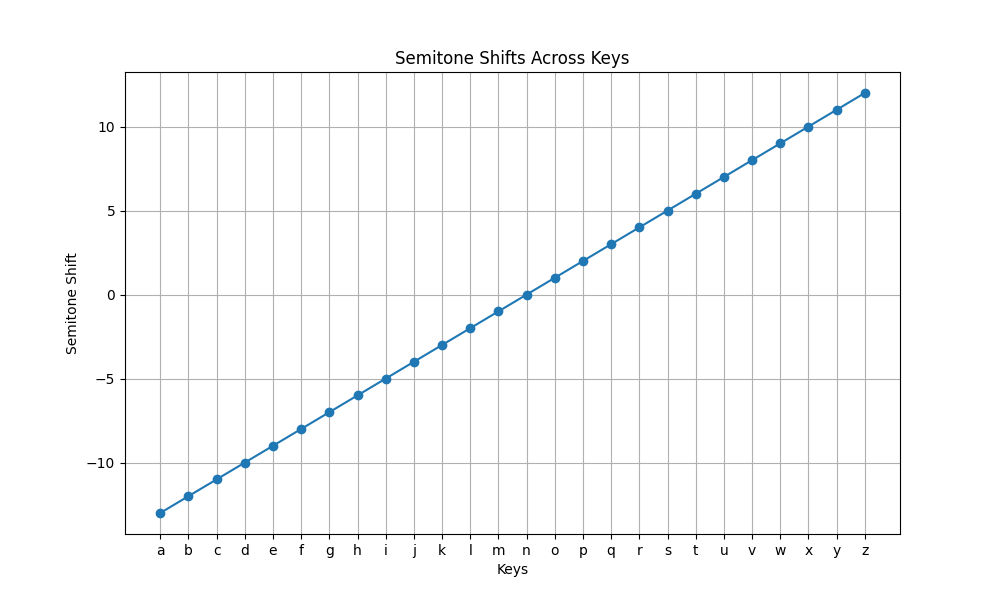
\includegraphics[width=0.8\textwidth]{Development/semitone_shifts.png}
\caption{Semitone shifts across keys from 'a' to 'z'.}
\end{figure} 




\subsubsection*{3. Application to Key Press Sounds}
For our virtual keyboard, we needed a unique pitch for each letter key (from 'a' to 'z'). We assigned a specific number of semitones to each key based on its position in the alphabet. The assignment is defined as follows:
\begin{equation}
s_i = i - 13
\end{equation}

where:
\begin{itemize}
  \item \( s_i \) is the pitch shift for the \( i \)-th letter,
  \item \( i \) is the index of the letter in the alphabet (0 for 'a', 25 for 'z').
\end{itemize}

\begin{figure}[h!]
\centering
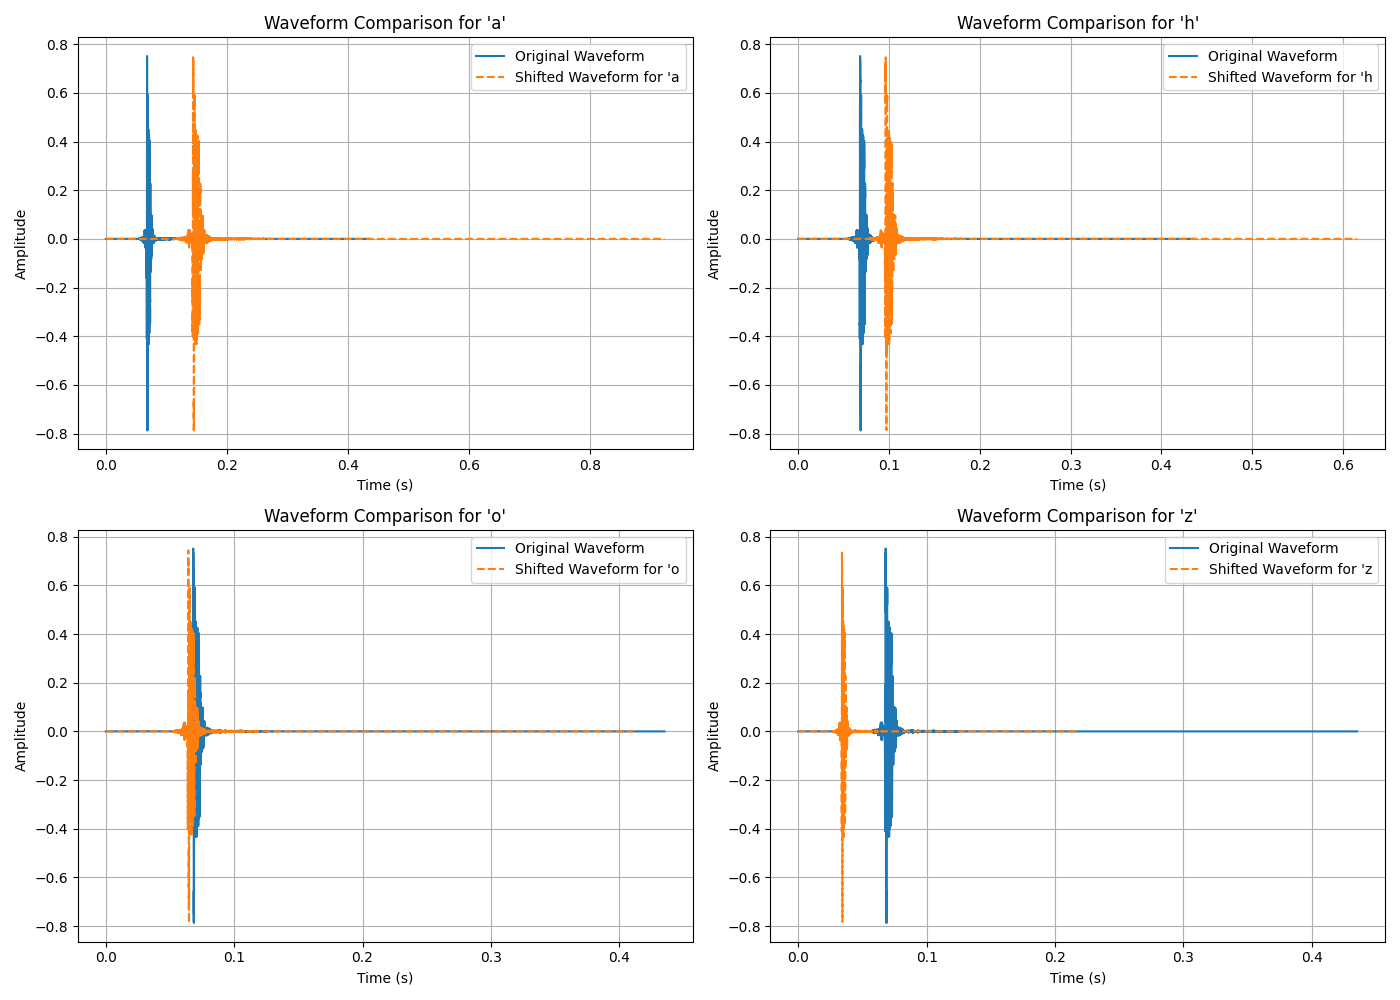
\includegraphics[width=0.8\textwidth]{Development/waveform_comparison_combined.png}
\caption{Waveform comparison of original and shifted sounds .}
\end{figure} 
\noindent \\\\\ \\ \\ 
This results in a pitch shift range from -13 semitones for 'a' to +12 semitones for 'z'.
By applying these mathematical principles of pitch shifting and sample rate adjustment, we generated distinct and responsive audio feedback for each key on a virtual keyboard. This method enhances the user experience by providing immediate and clear auditory confirmation of each key press, aligning with the principles of effective micro-interactions.

\subsection{Key Weight Calculation}
In the virtual keyboard simulation developed , we quantify the tactile feedback and the accuracy of the desired typed keys through a calculated "weight" assigned to each key and its respective parts. This weight metric plays a crucial role in simulating dynamic responses typical of physical keyboard interactions, which is essential for enhancing the accuracy of typing within the virtual environment. The need for such a simulation arises from the inherent discrepancies in the data frequencies between the frame rate of the virtual environment and the tracking system used for modeling hand movements. By synchronizing these elements through calculated key weights, we ensure that the user's interactions with the virtual keyboard are both intuitive and responsive, closely mimicking real-world typing experiences.


\subsubsection*{1. Key Part Weight Calculation}
The weight of each key part is determined based on its designated role and position within the key layout. For edge key parts, which are less frequently engaged during typing, a constant base weight is assigned, ensuring a uniform weight distribution for less significant key parts and is given by:
\begin{equation}
W_{\text{base}} = 0.1 \quad \text{(as an example value)}
\end{equation}
For central and more interactive key parts, the weight is dynamically calculated based on the key part's Cartesian coordinates on the keyboard grid. This method emphasizes the importance of centrally-located key parts:
\begin{equation}
W(x, y) = \frac{1}{\sqrt{(x - x_{\text{center}})^2 + (y - y_{\text{center}})^2 + 1}}
\end{equation}
where $x_{\text{center}}$ and $y_{\text{center}}$ represent the coordinates of the central key part of the keyboard, and the addition of 1 in the denominator prevents division by zero, ensuring that central key parts have the highest weights.

\subsubsection*{2. Overall Key Weight Calculation}
The total weight of a key at any moment is the sum of the weights of all its collided key parts. This sum is calculated periodically to determine the overall weight of the key:
\begin{equation}
W_{\text{key}} = \sum_{i=1}^{n} W_i
\end{equation}
where $W_i$ is the weight of the $i$-th collided key part. This cumulative weight is then used to identify the active key, which is the key with the highest total weight among all keys engaged at that instance.\\ \\
This approach models real-world typing by dynamically adjusting key sensitivity based on typical finger movements and interactions, thereby simulating an intuitive and realistic typing experience. The mathematical model ensures that the most probable key press is detected based on tactile feedback, which is crucial for providing accurate and responsive keyboard simulations.

\subsection*{3. Process Overview}
\begin{enumerate}
    \item \textbf{Collision Detection:} Each key part uses Unity's physics engine to detect collisions.
    \item \textbf{Event Notification:} Collisions trigger events that notify the parent key of the key part's status.
       \item \textbf{Register collided key:}
    The key notifies the keyboard upon activation and registers itself within the keyboard.
       
    \item \textbf{Weight Calculation:} The keyboard periodically checks all activated keys, aggregating the weights from their active key parts to calculate their total weights. It then identifies the key with the highest total weight
    
    \item \textbf{Key Press Detection:} A key is considered pressed if its aggregated weight is the highest among all keys.
    \item \textbf{Key Typed:} The determination of a key press is finalized when all collisions have ceased, particularly as the user lifts their finger from the key.
\end{enumerate}






















\chapter{Implementation of Typing Test Scenario and Metrics}

\section{Introduction}
This chapter details the implementation of a comprehensive typing test scenario designed to evaluate user performance with different virtual keyboard types in a virtual reality (VR) environment. The scenario includes various elements such as user input handling, data collection, phrase management, error tracking, and database integration to provide a robust framework for testing and analysis.

\section{Typing Test Scenario}

\subsection{Overview of the Typing Test Scenario}
The typing test scenario aims to assess the typing performance of users using different keyboard configurations in a VR environment. Specifically, the test compares the MRTK (Mixed Reality Toolkit) Keyboard with a custom virtual keyboard designed for this study. The MRTK Keyboard, part of Microsoft's Mixed Reality Toolkit, provides a standardized virtual input method that includes features such as spatial awareness, robust input handling, and support for hand and eye tracking \cite{mrtk_keyboard}. It is designed to facilitate ease of use and seamless interaction within virtual reality environments, making it an ideal choice for evaluating virtual text entry.
\begin{figure}[h]
    \centering
    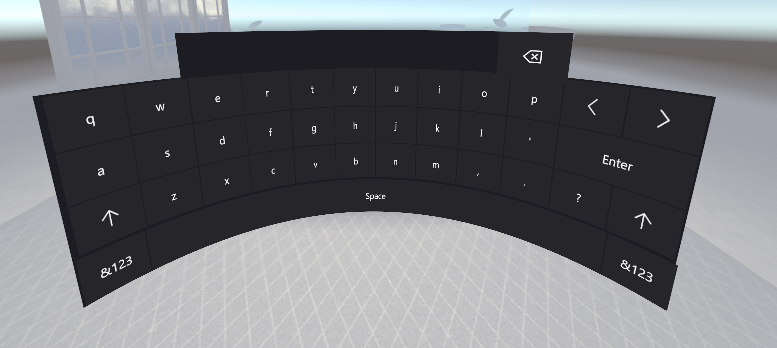
\includegraphics[width=0.8\textwidth]{Scenario/MRTK_KEyboard.PNG} % Replace with your image file name
    \caption{ \centering MRTK Keyboard interface showing a curved QWERTY layout designed for virtual reality environments inisde unity.}
    \label{fig:mrtk_keyboard}
\end{figure}\\ \\
The custom virtual keyboard, on the other hand, was created using Blender \ref{sec:Virtual Keyboard Conception} to incorporate enhanced haptic feedback mechanisms and ergonomic design tailored to improve user interaction and typing efficiency. This custom keyboard aims to address the limitations of existing virtual keyboards by providing a more intuitive and immersive typing experience through advanced haptic feedback and ergonomic considerations. 
\begin{figure}[h]
    \centering
    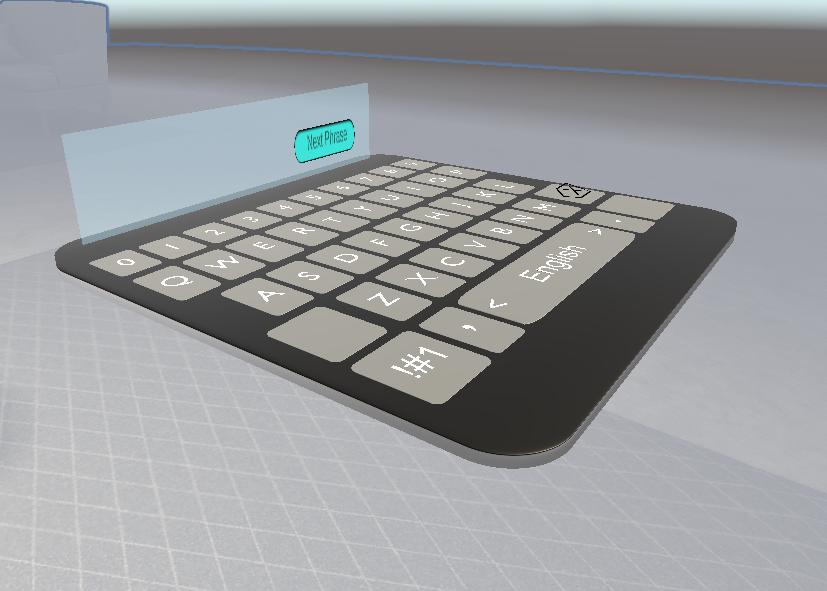
\includegraphics[width=0.8\textwidth]{Scenario/Custom_keyboard.PNG} % Replace with your image file name
    \caption{ \centering Custom virtual keyboard interface designed with enhanced haptic feedback and ergonomic features for improved typing efficiency in VR inside unity.}
    \label{fig:mrtk_keyboard}
\end{figure}\\ \\
The system captures detailed user input data, records performance metrics, and manages the flow of the test to ensure a comprehensive evaluation. The phrases used in the test are sourced from Scott MacKenzie's phrase sets, which are widely recognized in the field of text entry research. MacKenzie's phrase sets are designed to provide a standardized basis for evaluating text entry methods, featuring a wide range of commonly used words and phrases that reflect typical typing scenarios. These phrase sets are carefully curated to balance frequency and representativeness, ensuring that the typing tasks are both realistic and challenging \cite{mackenzie_phrase_set}. \\ \\
By using these standardized phrases, the study can reliably measure typing performance metrics such as Words Per Minute (WPM) and Error Rate (ER), providing valuable insights into the efficiency and accuracy of each keyboard configuration. The consistent use of MacKenzie's phrase sets allows for comparability with other studies in the field, facilitating a broader understanding of virtual text entry performance. 
\subsection{User Input Handling}
The system continuously monitors the user's typing input in a designated text field, tracking each keystroke and identifying any mistakes made during the typing process. This allows for real-time data collection and analysis of user performance.

\subsection{Data Collection}
Detailed data about the typing session is collected, including the time taken, the number of keystrokes, and the accuracy of the typed text compared to the expected text. After the user finishes typing a phrase, the system records this data and saves it inside a third-party database.

\subsection{Phrase Management}
The test involves typing a series of phrases. The system loads a new phrase for the user to type and displays it on the screen. Once the user finishes typing a phrase, the system prepares the next phrase, ensuring a continuous flow of the test.

\subsection{Error and Accuracy Tracking}
The system not only counts the total keystrokes but also keeps track of incorrect keystrokes, helping to measure the user's typing accuracy. It calculates various metrics such as error rate, accuracy in characters, accuracy in words, and typing speed.

\subsection{Interactive Elements}
Interactive elements such as a button allow the user to proceed to the next phrase. This ensures that users have control over the transition between different phrases and keyboard types.

\subsection{Data Storage}
All the typing data collected during the test is stored in a database. This data includes details like the typed text, the expected text, the time taken, and various accuracy metrics. Storing this data allows for detailed post-test analysis.

\subsection{Configuration and Setup}
Before starting the test, the system loads configuration settings such as the types of keyboards to be tested and other parameters that guide the test process. The configuration settings include:
\begin{itemize}
    \item Names of the keyboards to be tested.
    \item Number of phrases the user should type in both the training scene and the testing scene.
    \item Waiting duration between different keyboards of the test.
    \item Vibration and force feedback settings for the gloves.
\end{itemize}

\subsection{Scene Management}
The test scenario involves three main scenes: Training, Testing, and Waiting.
\begin{itemize}
    \item \textbf{Training Scene:} The user practices typing to get familiar with the keyboard.
    \item \textbf{Testing Scene:} The user is tested on their typing performance.
    \item \textbf{Waiting Scene:} The user waits while the system transitions between different keyboard types.
\end{itemize}

\subsection{Scene Occurrences}
For each keyboard, the sequence of scenes is:
\begin{enumerate}
    \item Training Scene
    \item Testing Scene
    \item Waiting Scene
\end{enumerate}

If we have 2 keyboards to test, the sequence repeats for each keyboard. Therefore, for 2 keyboards, the scenes will appear as follows:
\begin{itemize}
    \item Training Scene: 1 time per keyboard $\times$ 2 keyboards = 2 times
    \item Testing Scene: 1 time per keyboard $\times$ 2 keyboards = 2 times
    \item Waiting Scene: 1 time per 2 keyboards
\end{itemize}

\subsection{Adjustable Settings in the Database}
\begin{itemize}
    \item \textbf{Vibration and Force Feedback:} The vibration and force feedback settings of the gloves used in the test can be adjusted via the database. This ensures that the feedback experienced by the user is tailored to the specific requirements of the test scenario.
    \item \textbf{Waiting Duration:} The duration in seconds of the waiting period between different types of keyboards of the test can be adjusted in the database.
    \item \textbf{Keyboard Names:} The names and types of keyboards to be tested can be updated in the database, making the system adaptable to different testing needs.
    \item \textbf{Number of Phrases:} The number of phrases that the user is required to type in both the training and testing scenes can be configured in the database, ensuring the test is appropriately challenging and comprehensive.
\end{itemize}

\subsection{Detection of a Finished Phrase}
The system detects that a phrase is finished when the user types the expected number of words of the expected phrase to type and the phrase ends with a period. Upon detection, the system:
\begin{itemize}
    \item Records the typing data for the completed phrase.
    \item Makes the button for proceeding to the next phrase interactable.
\end{itemize}

\section{Workflow Summary}
The workflow of the typing test scenario involves the following steps:
\begin{enumerate}
    \item \textbf{Initialization:} The system sets up the test environment and prepares the first phrase.
    \item \textbf{Typing Phase:} The user types the displayed phrase, and the system tracks keystrokes and errors in real-time.
    \item \textbf{Detection of Completion:} The system detects when the user has finished typing the phrase by checking word count and punctuation.
    \item \textbf{Data Recording:} Upon completion of each phrase, the system records the typing data.
    \item \textbf{Phrase Transition:} The user moves to the next phrase by clicking a button.
    \item \textbf{Scene Transition:} The system transitions between Training, Testing, and Waiting scenes as needed for each keyboard type.
\end{enumerate}

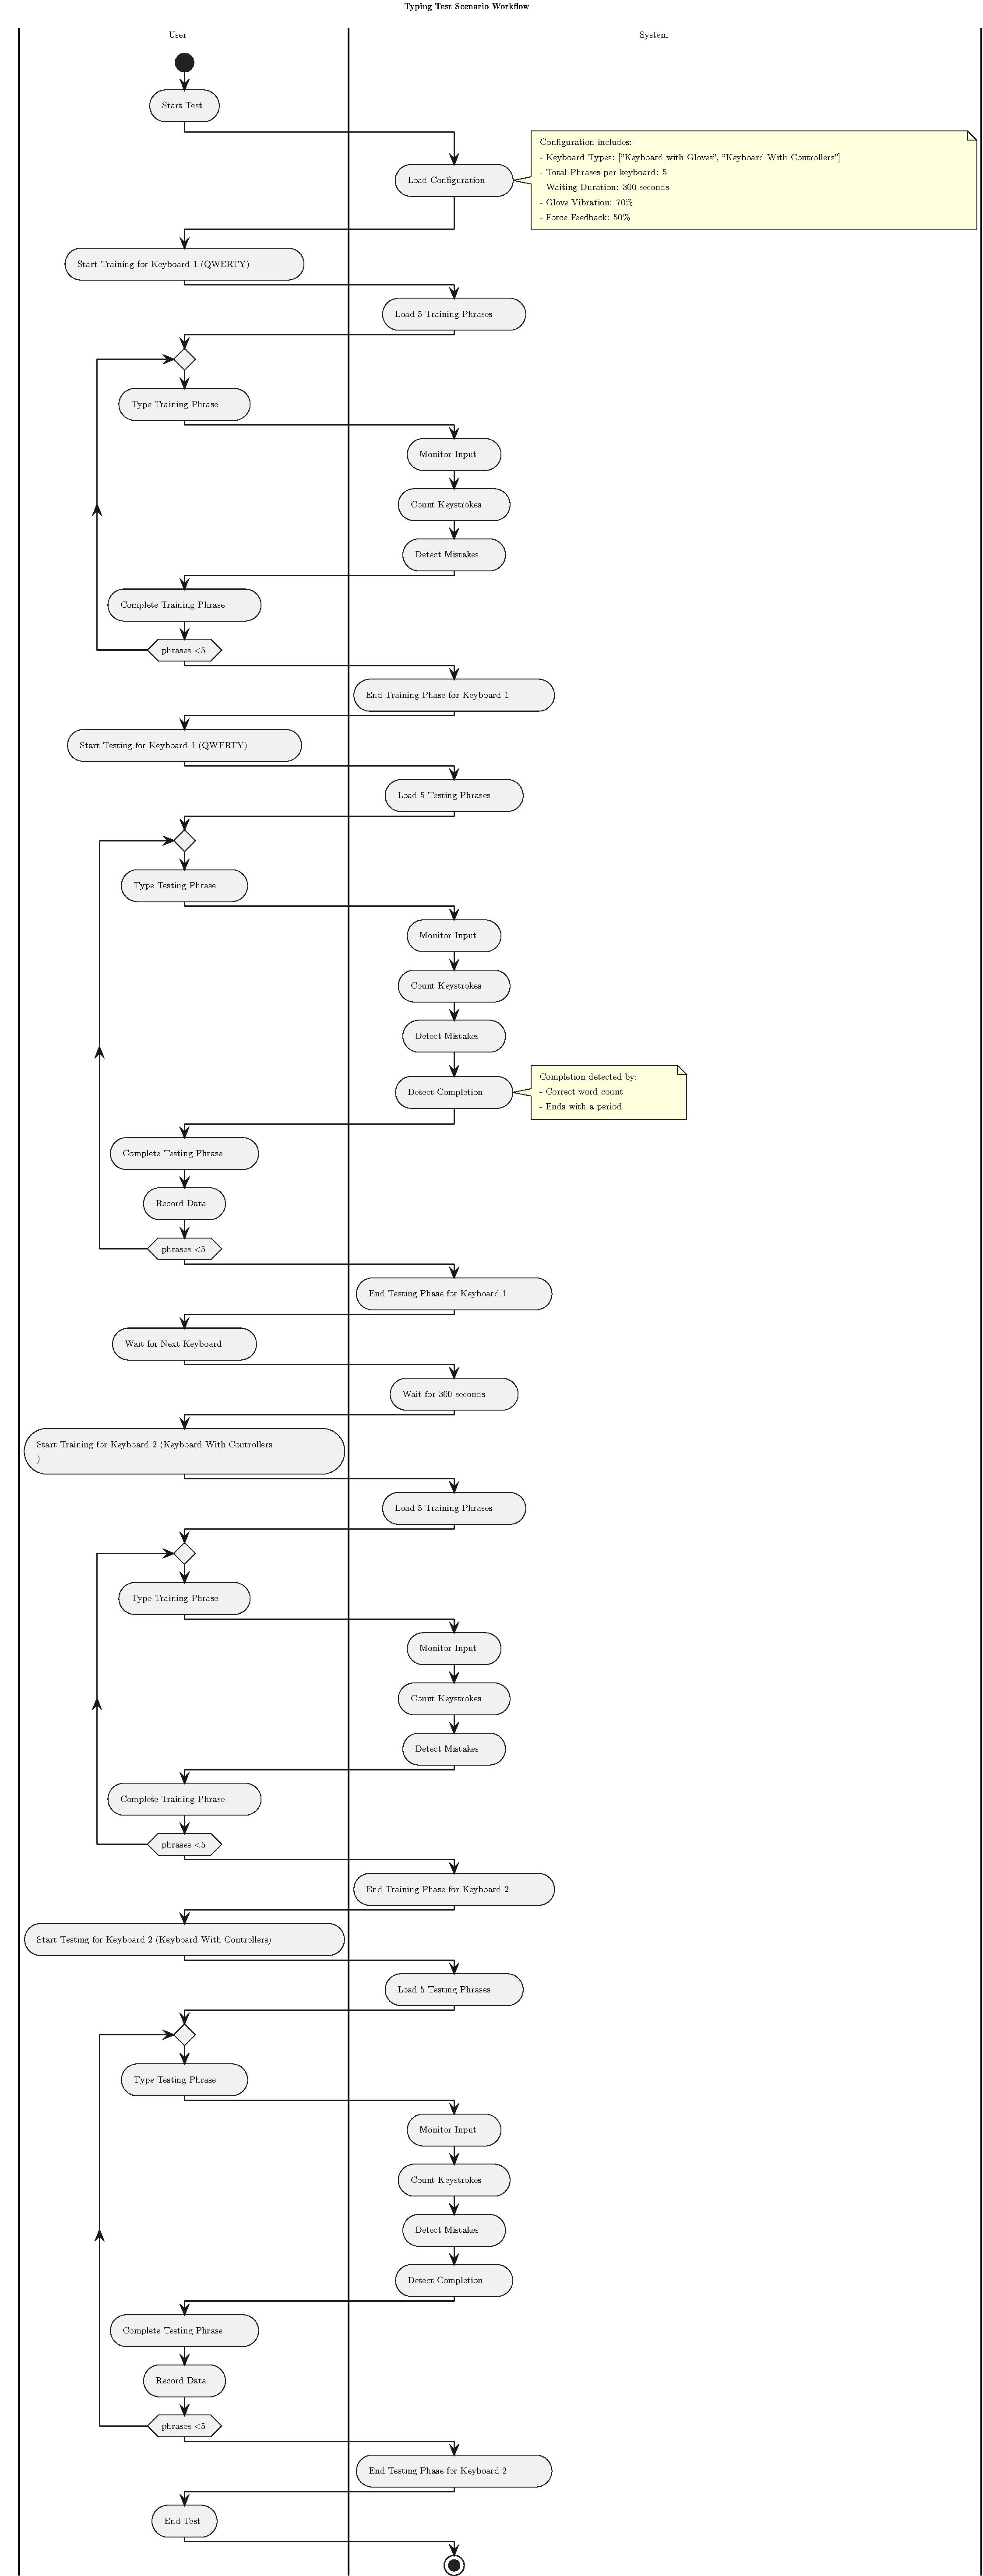
\includepdf[pages=-, landscape=true, fitpaper=true]{Scenario/scenario_PDF2.pdf}

\section{Typing Performance Metrics and Database Registration}

\subsection{Metrics Overview}
The performance of users is analyzed using several metrics. These metrics provide a comprehensive understanding of the user's typing efficiency and accuracy in the VR environment.

\begin{itemize}
    \item \textbf{Error Rate:} This metric calculates the percentage of errors by computing the Levenshtein distance between the expected text and the typed text. The Levenshtein distance \(d(s, t)\) is a measure of the minimum number of single-character edits (insertions, deletions, or substitutions) required to change one word into the other. The formula used to calculate the error rate is:
    \begin{equation}
    \text{Error Rate} = \frac{d(s, t)}{\max(\text{Length of Expected Text}, \text{Length of Typed Text})} \times 100
    \end{equation}
    where \(d(s, t)\) is the Levenshtein distance between the strings \(s\) (expected text) and \(t\) (typed text).

    \item \textbf{Character-Level Accuracy:} This metric measures the accuracy at the character level by calculating the Levenshtein distance and then determining the percentage of characters typed correctly. The formula used is:
    \begin{equation}
    \text{Accuracy in Characters} = 100 - \left( \frac{d(s, t)}{\text{Length of Expected Text}} \times 100 \right)
    \end{equation}
    This metric highlights the proportion of correctly typed characters relative to the expected characters.

    \item \textbf{Word-Level Accuracy:} This metric assesses the accuracy at the word level. It compares each word in the expected text with the corresponding word in the typed text, counting the mismatches. The formula used is:
    \begin{equation}
    \text{Accuracy in Words} = 100 - \left( \frac{\text{Number of Words with Errors}}{\text{Number of Words in Expected Text}} \times 100 \right)
    \end{equation}
    This metric provides insight into how accurately the user can reproduce words as opposed to individual characters.

    \item \textbf{Keystroke-Level Accuracy:} This metric evaluates the accuracy based on the number of incorrect keystrokes out of the total keystrokes made. The formula used is:
    \begin{equation}
    \text{Accuracy in Keystrokes} = 100 - \left( \frac{\text{Incorrect Keystrokes}}{\text{Total Keystrokes}} \times 100 \right)
    \end{equation}
    This metric helps in understanding the precision of each keystroke made by the user.

    \item \textbf{Typing Speed:} This metric calculates typing speed in words per minute (WPM). It assumes that an average word consists of five characters. The formula used is:
    \begin{equation}
    \text{Typing Speed} = \left( \frac{\text{Number of Characters Typed}}{5} \right) \div \left( \frac{\text{Time Taken in Seconds}}{60} \right)
    \end{equation}
    Typing speed is an important metric to gauge how quickly a user can type, which is crucial for evaluating productivity.

    \item \textbf{Keystrokes per Character:} This metric calculates the number of keystrokes per character typed. The formula used is:
    \begin{equation}
    \text{Keystrokes per Character} = \frac{\text{Keystroke Count}}{\max(1, \text{Character Count})}
    \end{equation}
    This metric indicates the efficiency of the user's typing, with a lower value signifying higher efficiency.

    \item \textbf{Levenshtein Distance:} The Levenshtein distance \(d(s, t)\) between two strings \(s\) and \(t\) is defined as the minimum number of single-character edits (insertions, deletions, or substitutions) required to transform \(s\) into \(t\). The distance can be computed using a dynamic programming approach where \(d(i, j)\) represents the distance between the first \(i\) characters of \(s\) and the first \(j\) characters of \(t\). The recursive formula is:
    \begin{equation}
    d(i, j) = \begin{cases} 
      i & \text{if } j = 0 \\
      j & \text{if } i = 0 \\
      \min \begin{cases} 
      d(i-1, j) + 1 \\ 
      d(i, j-1) + 1 \\ 
      d(i-1, j-1) + (1 - \text{match}(s_i, t_j))
      \end{cases} & \text{otherwise}
   \end{cases}
    \end{equation}
    Here, \(\text{match}(s_i, t_j)\) is 1 if the characters \(s_i\) and \(t_j\) are the same, and 0 otherwise. This metric provides a foundational measure of typing accuracy by quantifying how similar the typed text is to the expected text.
\end{itemize}

\subsection{Database Registration and Storage}
The application establishes a connection to the MongoDB database. This connection is initiated during the startup process, ensuring that the database connection is established when the application begins running. The necessary collections for storing user data and configuration settings are initialized at this point.

\subsubsection{Inserting Typing Data}
Typing performance data, encapsulated in a structured format, is inserted into the MongoDB collection. This data includes various metrics such as:
\begin{itemize}
    \item \textbf{Expected text:} The predefined text that the user is expected to type during the test.
    \item \textbf{Typed text:} The actual text that the user types, which is recorded for analysis.
    \item \textbf{Time taken to type:} The total time (in seconds) that the user takes to complete typing the expected text.
    \item \textbf{Keystroke count:} The total number of keystrokes made by the user during the typing session.
    \item \textbf{Error rate:} The percentage of errors made by the user, calculated using the Levenshtein distance between the expected text and the typed text.
    \item \textbf{Character-level accuracy:} The accuracy of the typed text at the character level, indicating how many characters were typed correctly relative to the expected text.
    \item \textbf{Word-level accuracy:} The accuracy of the typed text at the word level, indicating how many words were typed correctly relative to the expected text.
    \item \textbf{Keystroke-level accuracy:} The accuracy based on the number of incorrect keystrokes out of the total keystrokes made.
    \item \textbf{Typing speed:} The typing speed measured in words per minute (WPM), assuming an average word consists of five characters.
    \item \textbf{Keystrokes per character:} The number of keystrokes made per character typed, indicating the efficiency of the user's typing.
    \item \textbf{Session time:} The total duration of the typing session, from start to finish.
    \item \textbf{User ID:} A unique identifier for the user, used to track individual performance data.
    \item \textbf{Keyboard type:} The type of keyboard used by the user during the typing session, which could influence performance.
\end{itemize}

To illustrate the data collected during the typing test, we include two examples of documents stored in MongoDB. The first example shows a case where the phrase is typed correctly, and the second example shows a case where the phrase contains errors.

\begin{figure}[h]
    \centering
    \begin{subfigure}[b]{0.45\textwidth}
        \centering
        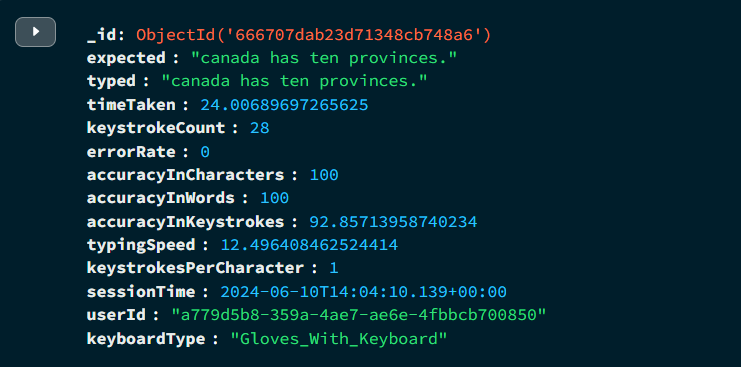
\includegraphics[width=\textwidth]{Scenario/Correct_Phrase.PNG}
        \caption{Correctly typed phrase}
        \label{fig:correct_case}
    \end{subfigure}
    \hfill
    \begin{subfigure}[b]{0.45\textwidth}
        \centering
        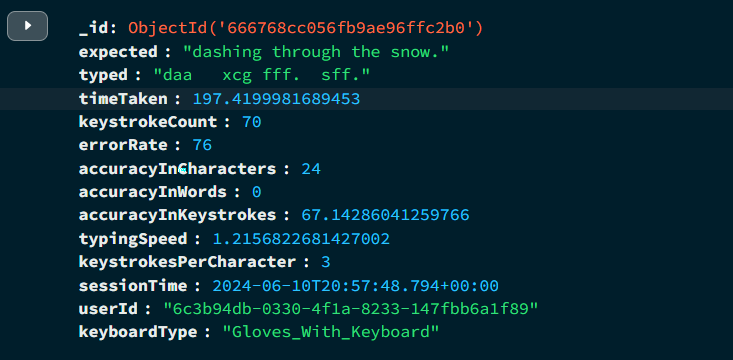
\includegraphics[width=\textwidth]{Scenario/wrong_Phrase.PNG}
        \caption{Incorrectly typed phrase}
        \label{fig:incorrect_case}
    \end{subfigure}
    \caption{Examples of typing data stored in MongoDB}
    \label{fig:database_examples}
\end{figure}

\subsubsection{Fetching Global Configuration}
Global configuration settings are retrieved from the database. The application queries the configuration collection and extracts various settings related to gloves configuration, keyboards to test, session settings, and waiting duration. These configurations are then used to adjust the application’s behavior based on the retrieved settings.

\subsubsection{Inserting User Data}
User data, encapsulated in a structured format, is inserted into the MongoDB collection. This data includes:
\begin{itemize}
    \item User ID
    \item User name
    \item User age
    \item User sex
\end{itemize}





\chapter{Conclusion} % (fold)
\label{sec:conclusion}

\ldots

% chapter conclusion (end)

\appendix
\bibliographystyle{plain}
\bibliography{ref}

\end{document}